\documentclass[11pt,a4paper]{article}

\usepackage[margin=1in]{geometry}
\usepackage[T1]{fontenc}
\usepackage{lmodern}
\usepackage{amsmath,amssymb}
\usepackage{graphicx}
\usepackage{booktabs}
\usepackage{longtable}
\usepackage{array}
\usepackage{xcolor}
\usepackage{algorithm}
\usepackage{algpseudocode}
\usepackage{caption}
\usepackage[numbers,sort&compress]{natbib}
\usepackage{microtype}
\usepackage[hidelinks]{hyperref}
\emergencystretch=2.5em

\captionsetup{font=small,labelfont=bf}
\graphicspath{{figures/}}
\setlength{\parskip}{0.35em}

\title{\textbf{Does Per-Cluster Resampler Selection Help?\\ ARS-Stack and a Controlled Evaluation of Adaptive Oversampling with Confidence-Weighted Ensembles on 28 Imbalanced Datasets}}
\author{Himansh Munjal\\ VIT, Vellore\\ \texttt{munjalhimansh2211@gmail.com}
\and Arnav Panwar\\ VIT, Vellore\\ \texttt{arnaw.panwar2023@vitstudent.ac.in}}
\date{}

\begin{document}
\maketitle

\begin{abstract}
Resampling methods for imbalanced classification, such as SMOTE, ADASYN, SMOTE-Tomek and SMOTE-ENN, are almost always applied \emph{uniformly} to the whole minority class, even though minority classes are often made of sub-regions with very different density and class overlap. We present \textbf{ARS-Stack} (Adaptive Resampler-Selection Stacking), which (i) clusters each minority class, (ii) scores every cluster by its class overlap and relative density, (iii) assigns each cluster the resampler suited to its local structure with a fixed, interpretable rule, (iv) applies that resampler locally under a global synthetic-sample budget, and (v) combines Random Forest, XGBoost and LightGBM with validation-AUC-PR confidence weights and a validation-tuned decision threshold. We also design a \emph{controlled} evaluation in which every resampling variant reaches the same class balance, so comparisons isolate \emph{which} resampler is used where rather than \emph{how much} data is added. On 28 datasets (credit-card fraud, mammography, 10-class yeast and 25 imbalanced-learn benchmarks; imbalance ratios 6--600), with 5-fold cross-validation repeated 3 times, nine variants, leakage-free nested validation, Nadeau--Bengio corrected $t$-tests, Holm correction and Friedman/Wilcoxon cross-dataset tests, ARS-Stack is statistically indistinguishable from global SMOTE, SMOTE-Tomek and no resampling (e.g.\ AUC-PR: 12 wins / 16 losses against SMOTE, Holm $p=0.88$). It is significantly better than global SMOTE-ENN (22/0/6 on AUC-PR and MCC, Holm $p<0.05$) and costs about 1.2$\times$ global SMOTE. Only 13 of 896 per-dataset tests are significant. Our analysis explains the result. Local cleaning touches only each cluster's majority neighbourhood, removing a median of 0\% of majority rows against 13.9\% for global SMOTE-ENN, so adaptive selection behaves like SMOTE. Validation-based confidence weights are close to uniform (median spread 0.022). We conclude that, with modern gradient-boosted ensembles and a tuned threshold, the choice of resampler matters much less than often assumed. We release a fully reproducible MLOps implementation.
\end{abstract}

\noindent\textbf{Keywords:} class imbalance, oversampling, SMOTE, cluster-based resampling, stacking ensembles, confidence weighting, statistical comparison of classifiers, reproducibility.

% =====================================================================
\section{Introduction}
% =====================================================================

\subsection{Motivation and Problem Context}

Many high-stakes classification problems are imbalanced: fraudulent card transactions are a fraction of a percent of all transactions \cite{dalpozzolo2015calibrating}, malignant calcifications are rare in mammography screening, and rare protein classes dominate the difficulty of biological prediction tasks. Standard learners trained to minimise overall error are biased toward the majority class and can reach high accuracy while missing most minority cases \cite{he2009learning}. The most widely used remedy is data-level resampling. SMOTE \cite{chawla2002smote} interpolates synthetic minority samples between minority neighbours. ADASYN \cite{he2008adasyn} focuses generation on hard-to-learn points. Hybrid methods such as SMOTE-Tomek and SMOTE-ENN \cite{batista2004study} add a cleaning step that removes noisy or overlapping samples. Over 85 SMOTE variants have been proposed \cite{fernandez2018smote,kovacs2019empirical}.

Almost all of these methods share a design assumption: one technique is applied \emph{globally} to the whole minority class. Real minority classes are rarely homogeneous. Fraud contains several distinct attack patterns, and a disease class contains sub-types with different presentations. A single minority class can therefore hold dense, well-separated clusters (where plain SMOTE suffices), clusters embedded in majority territory (where cleaning is needed to avoid amplifying noise), and sparse, isolated groups (where adaptive generation may help). This raises a natural question: \emph{should the resampler be chosen per local region of the minority class, rather than once per dataset?}

A second design choice concerns the classifier. Ensembles and stacking \cite{wolpert1992stacked,galar2012review} are the dominant way to combine resampling with strong learners. Gradient-boosted trees \cite{chen2016xgboost,ke2017lightgbm} are now the default base learners for tabular data. How the learners' predictions are combined, and at which decision threshold, also affects minority-class performance.

\subsection{Research Gaps}

From our review of the literature we identify five gaps that this work addresses.
\begin{enumerate}
  \item[\textbf{G1}] \textbf{Uniform resampling.} SMOTE variants and hybrid methods apply one technique to the whole minority class \cite{chawla2002smote,he2008adasyn,batista2004study}. Cluster-based methods \cite{douzas2018kmeanssmote} adapt \emph{how many} samples each region receives, but still use one generator everywhere. Choosing a \emph{different resampler} per minority cluster has not been systematically evaluated.
  \item[\textbf{G2}] \textbf{Confounded comparisons.} When resamplers are compared, each usually produces a different final class balance and a different training-set size. A difference in score can then come from the amount of oversampling rather than from the method itself.
  \item[\textbf{G3}] \textbf{Ensemble combination.} Stacking frameworks typically trust every base learner equally or fit a linear meta-learner. A linear meta-learner cancels any constant per-learner confidence scaling, so ``confidence weights'' fed into it are a no-op.
  \item[\textbf{G4}] \textbf{Fixed decision threshold.} Resampling shifts predicted probabilities, so the conventional 0.5 threshold is miscalibrated after oversampling. Many studies nevertheless report threshold-dependent metrics (F1, G-mean, MCC) at 0.5.
  \item[\textbf{G5}] \textbf{Weak statistical evidence.} Many proposals are validated on two or three datasets with a single split or with uncorrected cross-validation $t$-tests. These tests are known to have inflated Type-I error because CV training sets overlap \cite{nadeau2003inference}. Cross-dataset comparisons of the kind recommended by Dem{\v{s}}ar \cite{demsar2006statistical} and Benavoli et al.\ \cite{benavoli2016posthoc} remain rare.
\end{enumerate}

\subsection{Contributions}

\begin{enumerate}
  \item[\textbf{C1}] \textbf{ARS-Stack}, a per-cluster adaptive resampling method. It clusters each minority class, scores every cluster by class overlap and scale-free relative density, maps the scores to one of four resamplers with a fixed interpretable rule, and resamples each cluster locally under a global budget. It is followed by a confidence-weighted ensemble of Random Forest, XGBoost and LightGBM with a validation-tuned threshold (G1, G3, G4). The method handles binary and multiclass problems.
  \item[\textbf{C2}] \textbf{A budget-controlled ablation design.} All resampling variants reach the same target class balance. A weighted-average combiner makes confidence weights effective. Separate variants isolate (a) adaptive versus global resampling for each of the four resamplers, (b) confidence weighting versus equal weighting, (c) weighted averaging versus logistic-regression meta-stacking, (d) KMeans versus DBSCAN clustering, and (e) resampling versus none (G2).
  \item[\textbf{C3}] \textbf{A large, statistically rigorous evaluation.} We use 28 datasets, 9 variants, 5-fold CV repeated 3 times (3{,}780 fitted fold models), leakage-free nested validation, Nadeau--Bengio corrected $t$-tests with Holm correction per dataset, and Friedman/Iman--Davenport and Holm-corrected Wilcoxon tests across datasets (G5).
  \item[\textbf{C4}] \textbf{A mechanistic explanation of a largely negative result.} ARS-Stack matches SMOTE and no resampling and beats only global SMOTE-ENN. We trace this to two measurable effects: local cleaning barely changes the training set, and validation confidence weights are near-uniform.
  \item[\textbf{C5}] \textbf{An open, reproducible implementation} with data versioning (DVC), experiment tracking (MLflow), orchestration (Prefect), containerisation (Docker), REST serving (FastAPI), 112 unit tests, and code/configuration fingerprints that tie every result to the exact code that produced it.
\end{enumerate}

The rest of the paper is organised as follows. Section~\ref{sec:related} reviews related work. Section~\ref{sec:problem} formalises the problem, and Section~\ref{sec:method} describes ARS-Stack. Section~\ref{sec:verification} presents the verification methodology and Section~\ref{sec:setup} the experimental setup. Section~\ref{sec:results} reports and discusses the results, Section~\ref{sec:limitations} lists limitations, and Section~\ref{sec:conclusion} concludes.

% =====================================================================
\section{Related Work}\label{sec:related}
% =====================================================================

\subsection{SMOTE and Adaptive Synthetic Oversampling}

SMOTE \cite{chawla2002smote} generates a synthetic minority sample on the line segment between a minority point and one of its $k$ minority nearest neighbours. This avoids the over-fitting of random duplication, and SMOTE remains the reference oversampler. ADASYN \cite{he2008adasyn} weights each minority point by the fraction of majority points among its neighbours, so that more samples are generated where learning is hard. Borderline-SMOTE \cite{han2005borderline} restricts generation to minority points near the decision boundary. Fern{\'a}ndez et al.\ \cite{fernandez2018smote} survey more than 85 SMOTE extensions and single out \emph{within-class heterogeneity} (small disjuncts, overlap and noise) as an open challenge. All of these methods operate on the minority class as a whole; ARS-Stack instead chooses \emph{among} such generators per minority cluster.

\subsection{Hybrid Oversampling with Data Cleaning}

Batista et al.\ \cite{batista2004study} compare ten balancing methods on 13 UCI datasets. They introduce SMOTE-Tomek (SMOTE followed by removal of Tomek links) and SMOTE-ENN (SMOTE followed by Wilson's Edited Nearest Neighbours) and find the hybrid methods especially useful when classes overlap. Cleaning has a cost. ENN removes every sample whose neighbours mostly disagree with it, which can delete large parts of the majority class in overlapping data. Our results confirm this at scale: global SMOTE-ENN removes a median of 13.9\% and up to 92.6\% of majority rows (Table~\ref{tab:removed}). ARS-Stack uses cleaning only in clusters with high overlap and only on their local majority neighbourhood.

\subsection{Cluster-Based Oversampling}

K-means SMOTE \cite{douzas2018kmeanssmote} clusters the \emph{whole} input space, keeps clusters with a high minority share, and allocates synthetic samples to them in inverse proportion to their minority density. On 90 datasets it improves on SMOTE and other popular oversamplers. Like other cluster-based methods, it varies \emph{where and how many} samples are generated but always uses SMOTE as the generator. ARS-Stack is complementary. It clusters only the minority class, allocates the budget in proportion to cluster size, and varies the \emph{generator} by cluster.

\subsection{Ensembles and Stacking for Imbalanced Data}

Stacked generalisation \cite{wolpert1992stacked} trains a meta-learner on the out-of-fold predictions of base learners. Galar et al.\ \cite{galar2012review} review bagging-, boosting- and hybrid-based ensembles for class imbalance and show that combining data-level resampling with ensembles is usually stronger than either alone. Gradient-boosted tree libraries, XGBoost \cite{chen2016xgboost} and LightGBM \cite{ke2017lightgbm}, are among the strongest tabular learners and are routinely stacked with Random Forests. ARS-Stack uses these three heterogeneous learners. It compares a confidence-weighted average, an equal-weight average, and classic logistic-regression stacking under identical resampling.

\subsection{Empirical Comparisons and Statistical Methodology}

Kov{\'a}cs \cite{kovacs2019empirical} compares 85 oversampling variants on 104 datasets and finds that differences between well-designed oversamplers are often small, with no method uniformly best. On methodology, Dem{\v{s}}ar \cite{demsar2006statistical} recommends average ranks with the Friedman test (and the Iman--Davenport correction) followed by post-hoc tests, and the Wilcoxon signed-rank test for pairs of classifiers over many datasets. Benavoli et al.\ \cite{benavoli2016posthoc} show that mean-rank post-hoc tests depend on the other algorithms in the pool and recommend pairwise Wilcoxon tests instead. Within a single dataset, Nadeau and Bengio \cite{nadeau2003inference} show that the naive paired $t$-test on CV folds underestimates variance and propose a corrected resampled $t$-test. We follow all of these recommendations.

Table~\ref{tab:related} positions ARS-Stack against the closest prior work.

\begin{table}[t]\centering\small
\caption{Positioning of ARS-Stack relative to closely related work.}\label{tab:related}
\footnotesize\renewcommand{\arraystretch}{1.15}
\begin{tabular}{*{6}{>{\raggedright\arraybackslash}p{2.15cm}}}
\toprule
Work & Local adaptivity & Resampler varies locally & Noise cleaning & Ensemble & Evaluation scale \\
\midrule
SMOTE \cite{chawla2002smote} & no & no & no & no & 9 datasets \\
ADASYN \cite{he2008adasyn} & per point (weights) & no & no & no & 5 datasets \\
Borderline-SMOTE \cite{han2005borderline} & boundary points & no & no & no & small UCI study \\
SMOTE-Tomek/ENN \cite{batista2004study} & no & no & global & no & 13 datasets \\
K-means SMOTE \cite{douzas2018kmeanssmote} & per cluster (amount) & no & no & no & 90 datasets \\
Ensemble review \cite{galar2012review} & no & no & varies & yes & 44 datasets \\
\textbf{ARS-Stack (ours)} & per minority cluster & \textbf{yes} & local, only where overlap is high & weighted RF + XGB + LGBM & 28 datasets, 9 variants, 15 folds \\
\bottomrule
\end{tabular}
\end{table}

% =====================================================================
\section{Problem Formulation}\label{sec:problem}
% =====================================================================

Let $\mathcal{D}=\{(\mathbf{x}_i,y_i)\}_{i=1}^{N}$ with $\mathbf{x}_i\in\mathbb{R}^d$ and $y_i\in\mathcal{Y}=\{1,\dots,K\}$. Let $N_c$ be the number of samples of class $c$ and $c^\star=\arg\max_c N_c$ the majority class. The imbalance ratio is $\mathrm{IR}=N_{c^\star}/\min_c N_c$. For the binary case ($K=2$) we write $\mathcal{D}^+$ for the minority class and $\mathcal{D}^-$ for the majority class.

\paragraph{Resampling under a fixed budget.} Let the candidate resamplers be $\mathcal{R}=\{$\textsc{smote}, \textsc{adasyn}, \textsc{smote-tomek}, \textsc{smote-enn}$\}$. For a target balance ratio $\beta\in(0,1]$, every minority class $c\neq c^\star$ receives the synthetic budget
\begin{equation}
B_c=\max\!\big(0,\ \operatorname{round}(\beta N_{c^\star})-N_c\big).\label{eq:budget}
\end{equation}
A \emph{global} resampler $r\in\mathcal{R}$ generates $B_c$ samples for class $c$ with $r$. An \emph{adaptive} resampler partitions class $c$ into clusters $\{C_{c,1},\dots,C_{c,m_c}\}$, assigns each cluster a resampler $r_{c,j}=s(\phi(C_{c,j}))\in\mathcal{R}$ through a selection function $s$ of cluster descriptors $\phi$, and splits $B_c$ across the clusters. Fixing $B_c$ for every variant is the central control of this study (gap G2). Any performance difference between variants is then due to \emph{which} resampler is used \emph{where}, not to the amount of synthetic data.

\paragraph{Classification.} Given the resampled training set $\tilde{\mathcal{D}}$, base learners $h_1,\dots,h_L$ output class-probability estimates $p_\ell(\mathbf{x})$. These are combined into $\hat p(\mathbf{x})$ and, for binary tasks, thresholded at $\tau$:
\begin{equation}
\hat y(\mathbf{x})=\mathbb{1}\big[\hat p(\mathbf{x})\ge\tau\big].\label{eq:decision}
\end{equation}

\paragraph{Objective.} We seek the resampling strategy, combiner and threshold that maximise expected minority-sensitive performance $\mathbb{E}[M(\hat y, y)]$ on unseen data, for each metric $M$ among F1, AUC-PR, G-mean and MCC. Since $\mathbb{E}[M]$ is unknown, we estimate it by repeated stratified cross-validation and frame the study as four testable hypotheses:
\begin{itemize}
  \item[\textbf{H1}] Adaptive per-cluster resampler selection outperforms each global resampler at equal budget.
  \item[\textbf{H2}] Validation-AUC-PR confidence weighting outperforms an equal-weight average of the same learners.
  \item[\textbf{H3}] A confidence-weighted average performs at least as well as logistic-regression meta-stacking.
  \item[\textbf{H4}] Resampling (adaptive or global) outperforms training on the original distribution with a tuned threshold.
\end{itemize}
Table~\ref{tab:notation} summarises the notation.

\begin{table}[t]\centering\small
\caption{Notation.}\label{tab:notation}
\begin{tabular}{ll}
\toprule
Symbol & Meaning \\
\midrule
$N, d, K$ & number of samples, features, classes \\
$N_c$, $c^\star$ & size of class $c$; majority class \\
$C_{c,j}$, $m_c$ & $j$-th cluster of minority class $c$; number of clusters \\
$o_{c,j}$ & overlap score of a cluster (Eq.~\ref{eq:overlap}) \\
$\delta_{c,j}$, $\rho_{c,j}$ & density score and density ratio of a cluster (Eqs.~\ref{eq:density}--\ref{eq:ratio}) \\
$\theta_{\mathrm{vh}},\theta_{\mathrm{h}},\theta_{\rho}$ & selection thresholds: 0.70, 0.40, 0.75 \\
$\beta$, $B_c$, $b_{c,j}$ & target balance ratio; class budget; cluster allocation \\
$h_\ell$, $p_\ell$, $w_\ell$ & base learner, its probability estimate, its confidence weight \\
$\tau^\star$ & decision threshold tuned on the validation split \\
\bottomrule
\end{tabular}
\end{table}

% =====================================================================
\section{Proposed Method: ARS-Stack}\label{sec:method}
% =====================================================================

\subsection{Overview}

Figure~\ref{fig:arch} shows the full system. The \emph{data layer} (A) ingests the 28 datasets, removes exact duplicate rows before any split, and performs the stratified outer and inner splits. The scaler is fitted on the inner training split only. The \emph{adaptive resampling module} (B), the core contribution, clusters, scores, selects, allocates and resamples per minority cluster and merges the results into a balanced training set. The \emph{ensemble} (C) trains three heterogeneous learners on the balanced set, weights them by inner-validation AUC-PR, averages their probabilities and tunes the threshold. Layer (D) evaluates on the untouched outer test fold and serves the fitted model through a REST API. The MLOps layer (E) versions data, tracks runs, orchestrates the pipeline and fingerprints code and configuration.

\begin{figure}[t]\centering
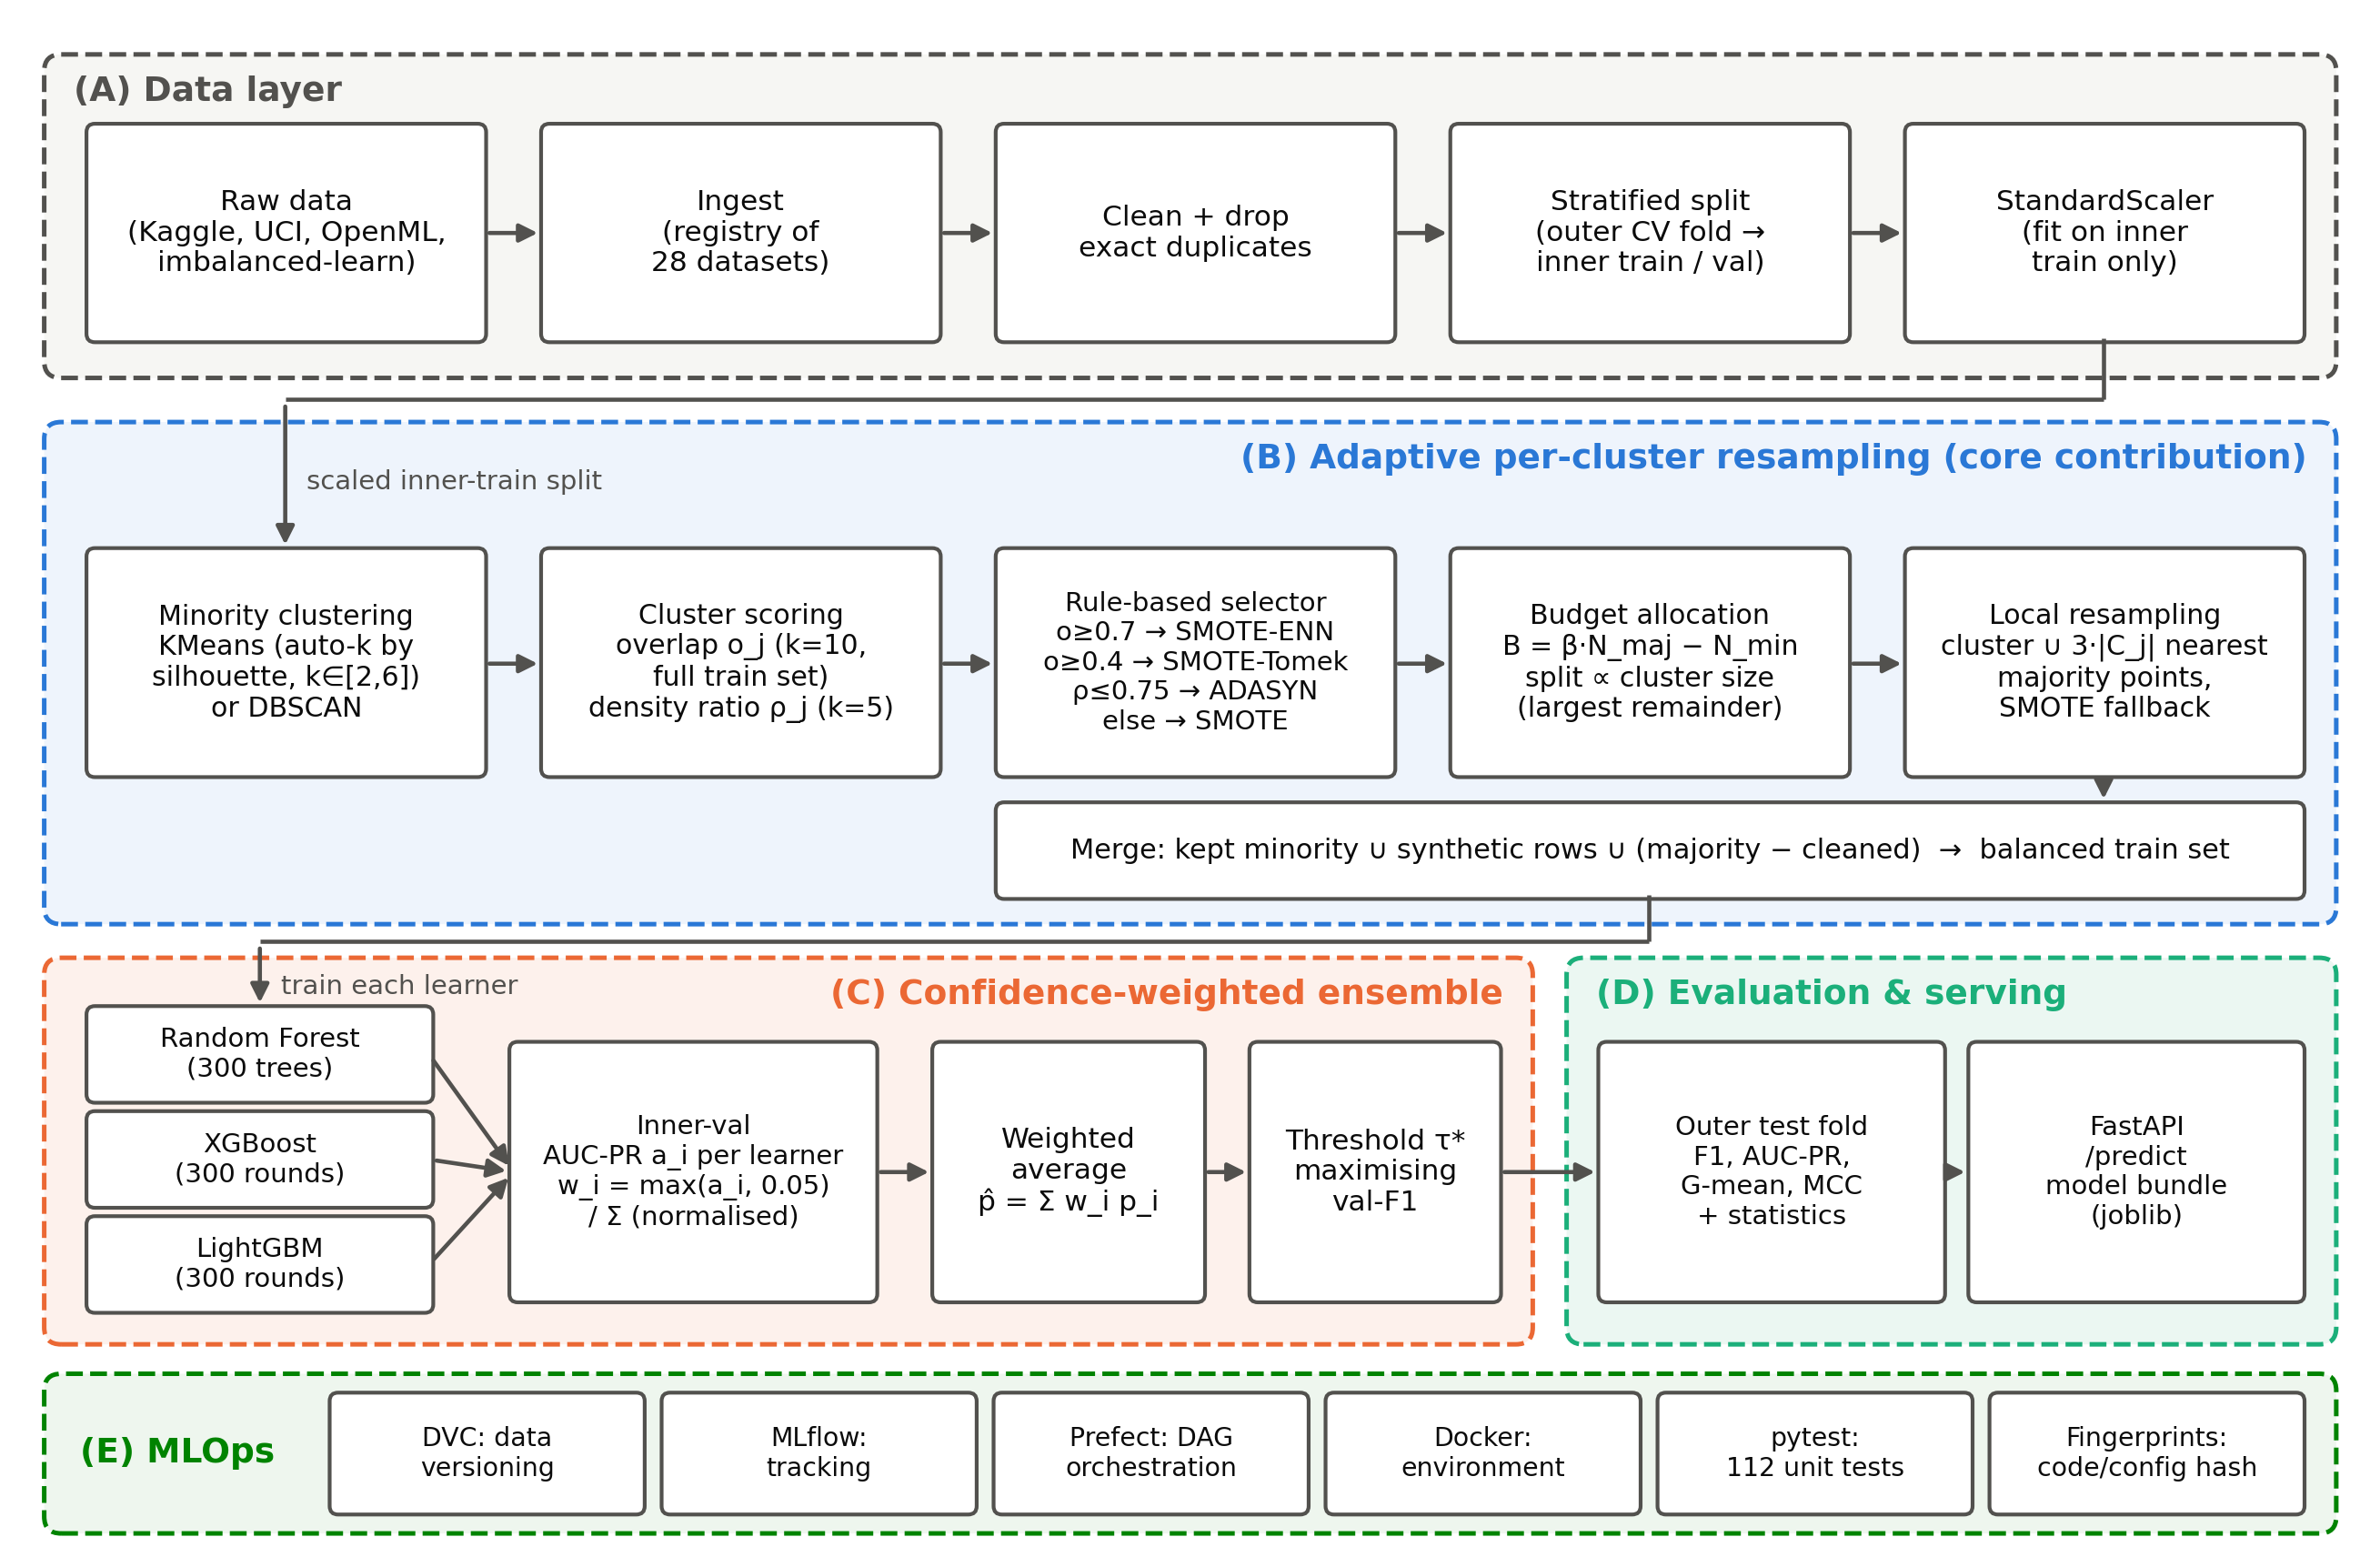
\includegraphics[width=\linewidth]{fig1_architecture.png}
\caption{ARS-Stack system architecture. (A) data layer; (B) adaptive per-cluster resampling, the core contribution; (C) confidence-weighted ensemble with threshold tuning; (D) evaluation and serving; (E) MLOps layer. All fitting in (A)--(C) uses only the inner training and validation splits of each outer fold.}
\label{fig:arch}
\end{figure}

\subsection{Minority-Class Clustering}

For each minority class $c$, the points $\mathbf{X}_c$ are clustered with KMeans. The number of clusters is chosen automatically as the $k\in[2,6]$ with the highest silhouette score (10 initialisations, fixed seed). DBSCAN ($\varepsilon=0.5$, $\mathrm{minPts}=5$) is available as an ablation, with its noise points relabelled as their own cluster rather than discarded. Three safety rules keep the downstream steps well defined:
(i) if $|\mathbf{X}_c|<2\cdot 10$, the class is treated as a single cluster;
(ii) any cluster with fewer than 10 points is merged into the largest cluster;
(iii) a cluster with fewer than 6 points (too few for $k=5$ SMOTE neighbours) is resampled by random oversampling.

\subsection{Cluster Scoring}

Each cluster is described by two quantities. The \emph{overlap score} is the mean fraction of majority points among the $k_o=10$ nearest neighbours of each cluster point, searched in the full training set (all classes):
\begin{equation}
o_{c,j}=\frac{1}{|C_{c,j}|}\sum_{\mathbf{x}\in C_{c,j}}\frac{1}{k_o}\sum_{\mathbf{z}\in\mathrm{NN}_{k_o}(\mathbf{x};\,\mathcal{D})}\mathbb{1}[y(\mathbf{z})\neq c]\ \in[0,1].\label{eq:overlap}
\end{equation}
The \emph{density score} is the inverse mean distance from each point to its $k_\delta=5$ nearest neighbours within the cluster:
\begin{equation}
\delta(C)=\Big(\frac{1}{|C|\,k_\delta}\sum_{\mathbf{x}\in C}\ \sum_{\mathbf{z}\in\mathrm{NN}_{k_\delta}(\mathbf{x};\,C\setminus\{\mathbf{x}\})}\lVert\mathbf{x}-\mathbf{z}\rVert_2\Big)^{-1}.\label{eq:density}
\end{equation}
Raw density depends on the feature scale of each dataset, so a fixed cutoff on it would not transfer between datasets. We therefore use the scale-free \emph{density ratio}
\begin{equation}
\rho_{c,j}=\delta(C_{c,j})\,/\,\delta(\mathbf{X}_c),\label{eq:ratio}
\end{equation}
where $\rho=1$ means the cluster is as dense as its class as a whole and $\rho<1$ means it is sparser.

\subsection{Resampler Selection Rule}

Each cluster receives a resampler through a fixed decision rule (Figure~\ref{fig:rule}):
\begin{equation}
s(o,\rho)=\begin{cases}
\textsc{smote-enn} & \text{if } o\ge\theta_{\mathrm{vh}}=0.70 \quad\text{(strong overlap: aggressive cleaning)}\\
\textsc{smote-tomek} & \text{if } \theta_{\mathrm{h}}=0.40\le o<0.70 \quad\text{(moderate overlap: boundary cleaning)}\\
\textsc{adasyn} & \text{if } o<0.40 \text{ and } \rho\le\theta_\rho=0.75 \quad\text{(sparse cluster)}\\
\textsc{smote} & \text{otherwise} \quad\text{(well-behaved cluster).}
\end{cases}\label{eq:rule}
\end{equation}
The rule follows the rationale of the original methods. Cleaning hybrids target overlap \cite{batista2004study}, ADASYN targets hard and sparse regions \cite{he2008adasyn}, and SMOTE is the default \cite{chawla2002smote}. The thresholds are absolute and interpretable. Overlap is already on a fixed $[0,1]$ scale, and density is expressed relative to the class. All three thresholds were fixed \emph{a priori}, before any result was produced, and were never tuned on test folds. A percentile-based (relative) mode exists in the code but is disabled by default: with only 1--2 clusters, percentiles force a choice by rank instead of by structure.

\begin{figure}[t]\centering
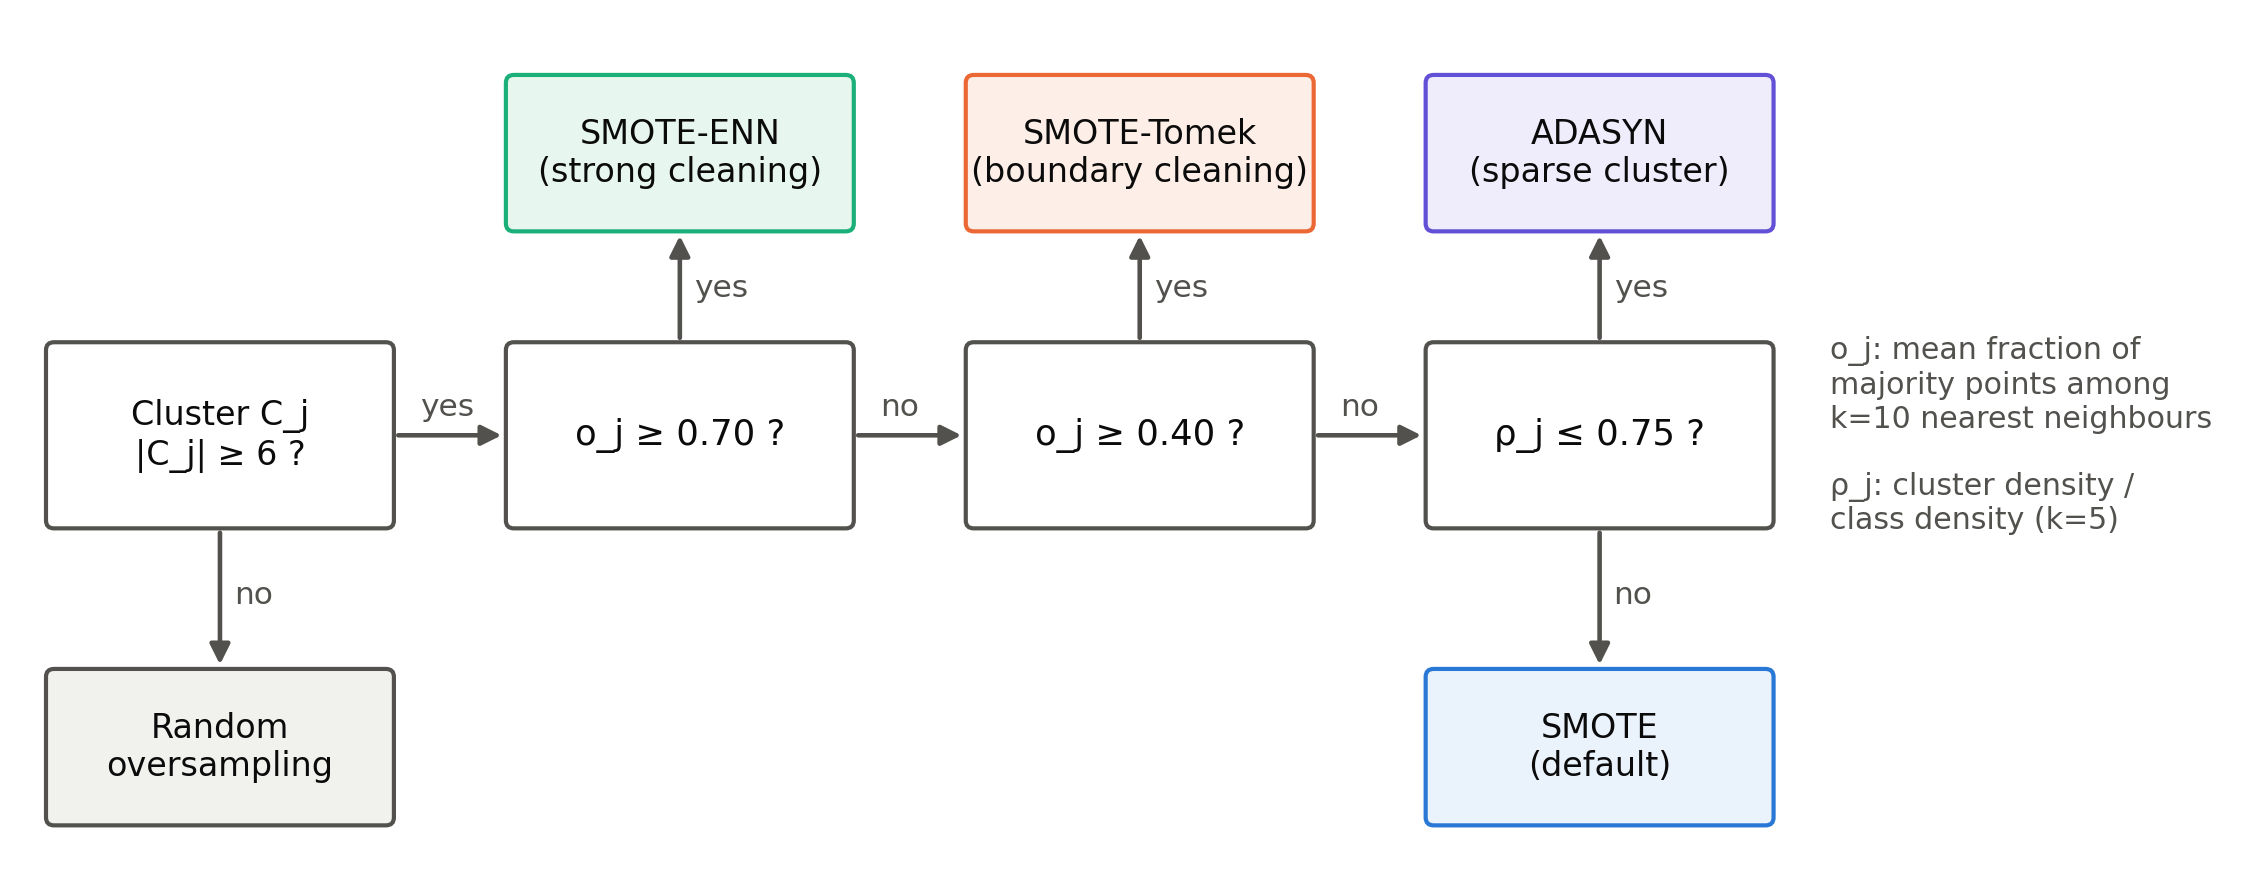
\includegraphics[width=0.92\linewidth]{fig2_selection_rule.png}
\caption{Per-cluster resampler selection rule (Eq.~\ref{eq:rule}).}
\label{fig:rule}
\end{figure}

\subsection{Budget Allocation}

The class budget $B_c$ (Eq.~\ref{eq:budget}) is split across clusters in proportion to cluster size, using largest-remainder rounding so that the parts sum exactly to $B_c$:
\begin{equation}
b_{c,j}=\Big\lfloor B_c\tfrac{|C_{c,j}|}{N_c}\Big\rfloor+\epsilon_{c,j},\qquad \epsilon_{c,j}\in\{0,1\},\qquad \sum_j b_{c,j}=B_c.\label{eq:alloc}
\end{equation}
Every global baseline uses the same $\beta$ (here $\beta=1$, full balance), so all resampling variants are compared at an equal synthetic budget.

\subsection{Local Resampling with Majority Context}

The chosen resampler for cluster $C_{c,j}$ is fitted on a \emph{local} problem: the cluster's minority points together with the $k_m=\max(3|C_{c,j}|,10)$ majority points nearest to the cluster centroid. This context gives SMOTE-Tomek and SMOTE-ENN the majority neighbours they need to detect boundary noise, and gives ADASYN a non-trivial difficulty signal. The resampler is asked to produce exactly $|C_{c,j}|+b_{c,j}$ minority points. If it fails (for example, ADASYN finds no majority neighbours), SMOTE produces the same number of samples instead. This fallback was triggered for 0.5\% of clusters. The final training set is the union of the retained minority points, all synthetic points, and the majority class minus any majority points that a cleaning resampler removed from a local context.

\subsection{Multiclass Extension}

For $K>2$ (Figure~\ref{fig:multiclass} in the Appendix), each non-majority class $c$ is processed independently one-vs-rest. It receives its own budget $B_c$, its own clustering, and overlap scores computed with ``not $c$'' as the opposing class. Its own per-cluster resamplers are then applied. Metrics and confidence weights use macro-averages.

\subsection{Confidence-Weighted Ensemble and Threshold Tuning}

Three heterogeneous learners are trained on $\tilde{\mathcal{D}}$: Random Forest (300 trees), XGBoost \cite{chen2016xgboost} and LightGBM \cite{ke2017lightgbm} (300 rounds each, learning rate 0.1, depth 6 for XGBoost). Let $a_\ell$ be the AUC-PR of learner $\ell$ on the inner validation split (macro AUC-PR for multiclass). The confidence weights are
\begin{equation}
w_\ell=\frac{\max(a_\ell,\,w_{\min})}{\sum_{m}\max(a_m,\,w_{\min})},\qquad w_{\min}=0.05,\label{eq:weights}
\end{equation}
and the ensemble probability is the weighted average $\hat p(\mathbf{x})=\sum_\ell w_\ell\, p_\ell(\mathbf{x})$. We deliberately use a weighted \emph{average} rather than a meta-learner. A logistic-regression meta-learner would absorb any constant rescaling of its inputs into its own coefficients, so weighting its inputs would have no effect (gap G3). For binary tasks, the decision threshold maximises F1 on the validation split:
\begin{equation}
\tau^\star=\arg\max_{\tau}\ \mathrm{F1}\big(y_{\mathrm{val}},\ \mathbb{1}[\hat p(\mathbf{X}_{\mathrm{val}})\ge\tau]\big),\label{eq:threshold}
\end{equation}
evaluated at every distinct validation probability. AUC-PR is threshold-free; F1, G-mean and MCC are computed at $\tau^\star$.

\subsection{Algorithm and Complexity}

Algorithm~\ref{alg:ars} summarises training. Clustering with automatic $k$ costs $O(5\cdot n_{\mathrm{init}}\cdot N_c\,k\,d\,T)$ for KMeans plus $O(N_c^2)$ for each silhouette evaluation. Overlap scoring needs one $k_o$-NN query per minority point against the training set. Local resampling operates on at most $4|C_{c,j}|$ (plus budget) points per cluster. Because the minority class is small, the adaptive step adds little to ensemble training. Its median fold time is $1.20\times$ that of global SMOTE (Table~\ref{tab:cost}). On credit card it is about $110\times$ \emph{faster} than global SMOTE-Tomek or SMOTE-ENN resampling, because cleaning runs only on local neighbourhoods instead of the 192{,}000-row majority class.

%ALG-BEGIN
\begin{algorithm}[t]
\caption{ARS-Stack training on one (inner) training split}\label{alg:ars}
\begin{algorithmic}[1]
\Require training split $(\mathbf{X},\mathbf{y})$, validation split $(\mathbf{X}_v,\mathbf{y}_v)$, balance ratio $\beta$
\State fit scaler on $\mathbf{X}$; transform $\mathbf{X}$ and $\mathbf{X}_v$
\State $\tilde{\mathcal{D}}\gets$ majority class $c^\star$
\For{each class $c\neq c^\star$}
  \State $B_c\gets\max(0,\operatorname{round}(\beta N_{c^\star})-N_c)$ \Comment{Eq.~\ref{eq:budget}}
  \State $\{C_{c,j}\}\gets$ \textsc{Cluster}$(\mathbf{X}_c)$ \Comment{KMeans, $k$ by silhouette}
  \For{each cluster $C_{c,j}$}
    \State $o\gets$ overlap$(C_{c,j})$;\ $\rho\gets$ density ratio$(C_{c,j})$ \Comment{Eqs.~\ref{eq:overlap}--\ref{eq:ratio}}
    \State $r\gets s(o,\rho)$; $b_{c,j}\gets$ allocation \Comment{Eqs.~\ref{eq:rule}, \ref{eq:alloc}}
    \State $M\gets k_m$ majority points nearest to centroid$(C_{c,j})$
    \State $(S, M')\gets r.\textsc{FitResample}(C_{c,j}\cup M)$ to $|C_{c,j}|+b_{c,j}$ minority points (SMOTE fallback)
    \State add retained minority and synthetic points $S$ to $\tilde{\mathcal{D}}$; mark $M\setminus M'$ as removed
  \EndFor
\EndFor
\State remove marked majority points from $\tilde{\mathcal{D}}$
\State train RF, XGBoost, LightGBM on $\tilde{\mathcal{D}}$
\State $w_\ell\gets$ normalised validation AUC-PR \Comment{Eq.~\ref{eq:weights}}
\State $\tau^\star\gets$ F1-optimal threshold of $\sum_\ell w_\ell p_\ell$ on the validation split \Comment{Eq.~\ref{eq:threshold}}
\State \Return $(\text{scaler},\{h_\ell\},\{w_\ell\},\tau^\star)$
\end{algorithmic}
\end{algorithm}
%ALG-END

% =====================================================================
\section{Verification Method}\label{sec:verification}
% =====================================================================

We verify ARS-Stack at two levels. \emph{Empirical verification} tests hypotheses H1--H4 with a controlled, leakage-free and statistically corrected protocol. \emph{Implementation verification} checks that the code does what the method specifies.

\subsection{Leakage-Free Nested Evaluation Protocol}

Figure~\ref{fig:protocol} shows the protocol. Each dataset is first deduplicated. It is then split by repeated stratified $K$-fold cross-validation into 5 folds, repeated 3 times with seed 42, giving 15 paired outer folds. All variants see exactly the same folds. Within each outer training portion, a stratified 15\% inner validation split is held out. The scaler, the resampler and the base learners are fitted on the remaining 85\%. The confidence weights and the decision threshold are chosen on the inner validation split, and all metrics are computed on the untouched outer test fold. No test-fold information enters any fitted component, and no synthetic sample is ever evaluated.

\begin{figure}[t]\centering
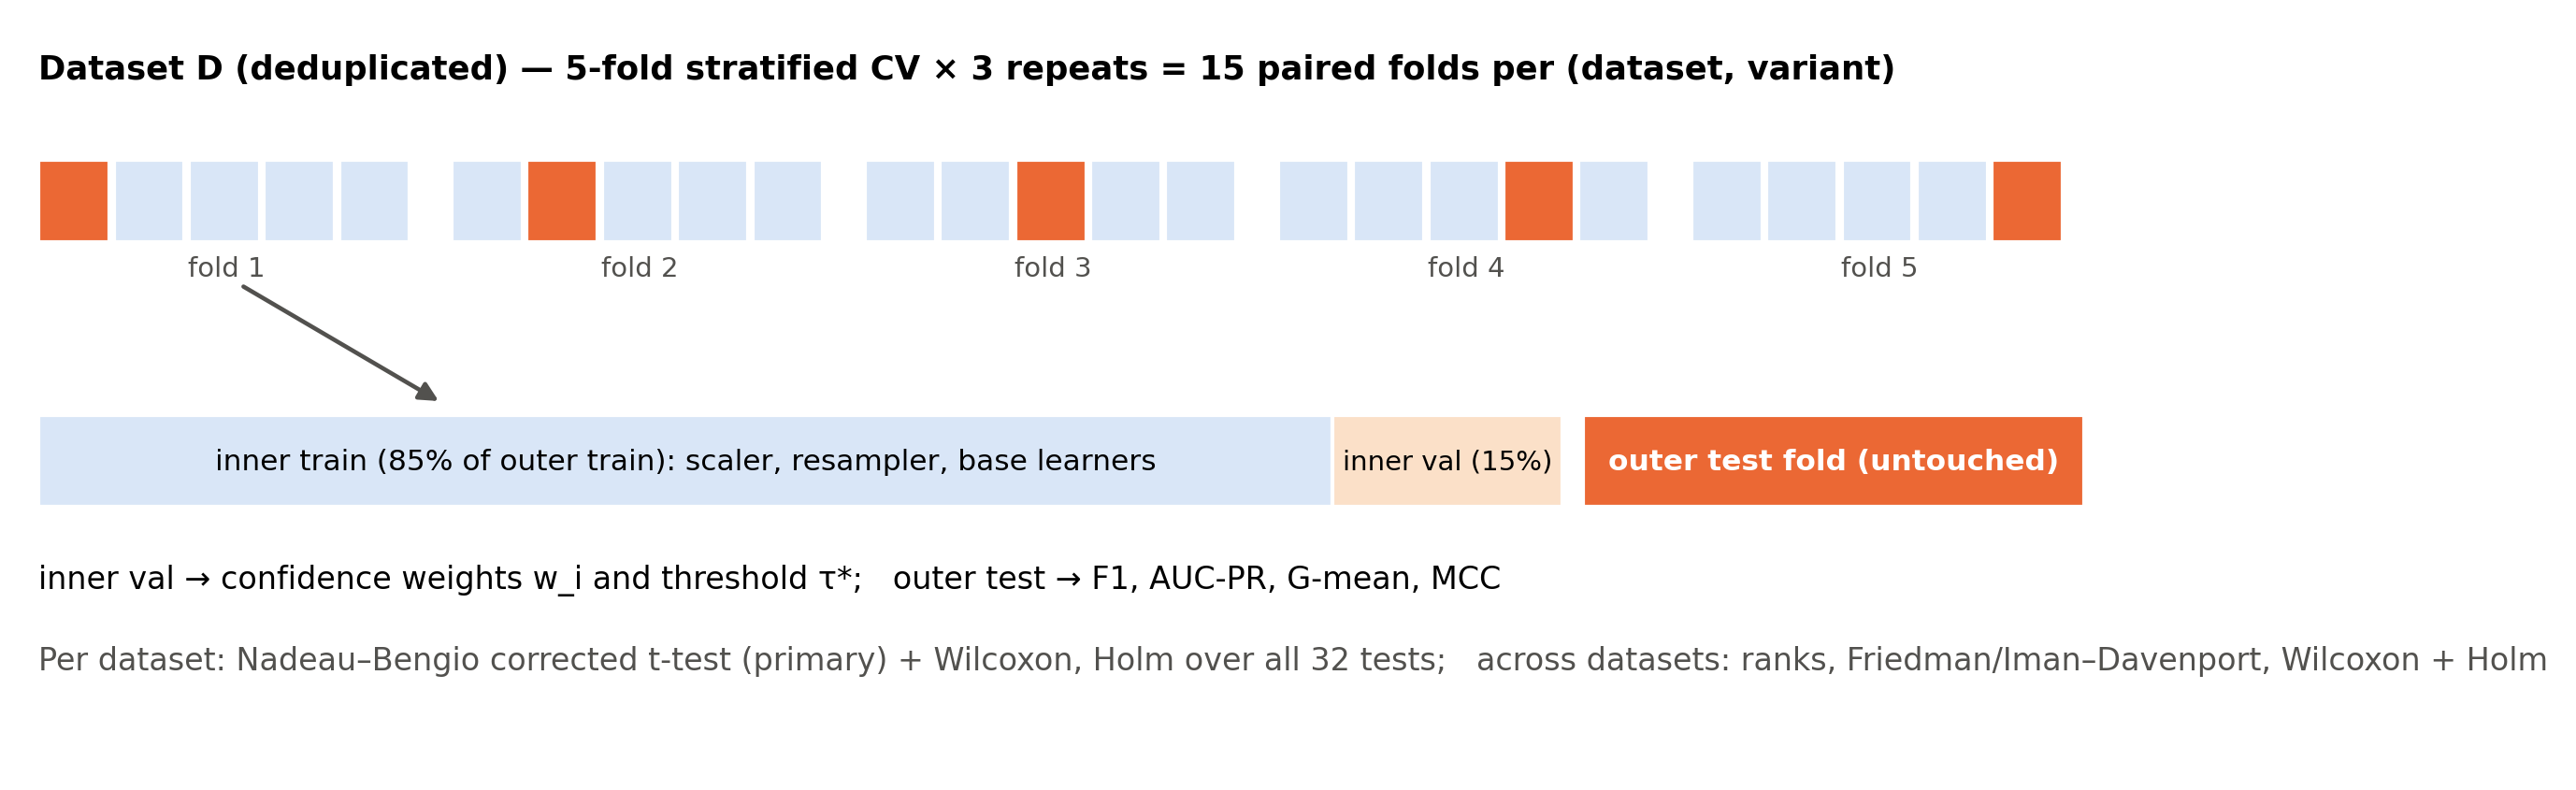
\includegraphics[width=\linewidth]{fig3_protocol.png}
\caption{Leakage-free nested evaluation protocol. Orange: outer test fold of the current iteration.}
\label{fig:protocol}
\end{figure}

\subsection{Controlled Ablation Variants}

Table~\ref{tab:variants} lists the nine variants. Each changes exactly one component of ARS-Stack, so each paired comparison isolates one design decision.

\begin{table}[t]\centering\small
\caption{The nine evaluated variants. Every resampling variant uses the same target balance $\beta=1$ and the same ensemble, threshold tuning and folds.}\label{tab:variants}
\footnotesize
\begin{tabular}{lll}
\toprule
Variant & Change relative to ARS-Stack & Isolates \\
\midrule
\textbf{ARS-Stack} & --- (adaptive KMeans + confidence-weighted average) & --- \\
Equal-weight avg. & $w_\ell=1/3$ & confidence weighting (H2) \\
LR meta-stacking & LR meta-learner on 5-fold out-of-fold probabilities & combiner (H3) \\
ARS (DBSCAN) & DBSCAN instead of KMeans & clustering robustness \\
SMOTE & one global SMOTE & adaptive selection (H1) \\
ADASYN & one global ADASYN & adaptive selection (H1) \\
SMOTE-Tomek & one global SMOTE-Tomek & adaptive selection (H1) \\
SMOTE-ENN & one global SMOTE-ENN & adaptive selection (H1) \\
No resampling & original class distribution & value of resampling (H4) \\
\bottomrule
\end{tabular}
\end{table}

\subsection{Evaluation Metrics}

Accuracy is uninformative under imbalance \cite{he2009learning}, so we report four minority-sensitive metrics. With TP, FP, TN and FN counted for the minority (positive) class:
\begin{gather}
\mathrm{F1}=\frac{2\,\mathrm{TP}}{2\,\mathrm{TP}+\mathrm{FP}+\mathrm{FN}},\qquad
\text{G-mean}=\sqrt{\frac{\mathrm{TP}}{\mathrm{TP}+\mathrm{FN}}\cdot\frac{\mathrm{TN}}{\mathrm{TN}+\mathrm{FP}}},\\
\mathrm{MCC}=\frac{\mathrm{TP}\cdot\mathrm{TN}-\mathrm{FP}\cdot\mathrm{FN}}{\sqrt{(\mathrm{TP}+\mathrm{FP})(\mathrm{TP}+\mathrm{FN})(\mathrm{TN}+\mathrm{FP})(\mathrm{TN}+\mathrm{FN})}},
\end{gather}
and AUC-PR is computed as average precision, $\mathrm{AP}=\sum_n (R_n-R_{n-1})P_n$, over the ranked predicted probabilities. AUC-PR is the primary metric because it is threshold-free and focuses on the minority class. For the 10-class yeast dataset, all four metrics are macro-averaged.

\subsection{Statistical Tests}

\paragraph{Within a dataset.} For each of the 8 comparisons (ARS-Stack versus each other variant) and 4 metrics, we have 15 paired fold differences $d_1,\dots,d_n$. The primary test is the Nadeau--Bengio corrected resampled $t$-test \cite{nadeau2003inference}, which inflates the variance to account for overlapping training sets:
\begin{equation}
t=\frac{\bar d}{\sqrt{\big(\frac{1}{n}+\frac{n_{\mathrm{test}}}{n_{\mathrm{train}}}\big)\,\hat\sigma_d^2}},\qquad \frac{n_{\mathrm{test}}}{n_{\mathrm{train}}}=\frac{1}{k-1}=\frac14,\qquad \mathrm{df}=n-1.\label{eq:nb}
\end{equation}
The Wilcoxon signed-rank test is reported alongside. The effect size is the matched-pairs rank-biserial correlation. Holm's step-down correction is applied over all $8\times4=32$ tests of a dataset.

\paragraph{Across datasets.} Following \cite{demsar2006statistical,benavoli2016posthoc}, each variant is ranked on every dataset by its mean score (ties receive average ranks). We test the null hypothesis that all variants are equivalent with the Friedman statistic and its Iman--Davenport $F$ correction,
\begin{equation}
\chi_F^2=\frac{12D}{J(J+1)}\Big[\sum_{j}R_j^2-\frac{J(J+1)^2}{4}\Big],\qquad F_{ID}=\frac{(D-1)\chi_F^2}{D(J-1)-\chi_F^2},\label{eq:friedman}
\end{equation}
with $D=28$ datasets, $J=9$ variants and average ranks $R_j$. ARS-Stack is then compared with each variant by a Wilcoxon signed-rank test over the 28 per-dataset means, Holm-corrected within each metric. This avoids the pool-dependence of mean-rank post-hoc tests \cite{benavoli2016posthoc}.

\subsection{Implementation Verification and Reproducibility Controls}

\begin{itemize}
  \item \textbf{Unit tests.} 112 \texttt{pytest} tests over seven modules check clustering fallbacks, overlap and density scores on synthetic geometries, the selection rule at each threshold boundary, exact budget allocation, multiclass resampling, weight normalisation and threshold tuning, metric correctness, the statistical tests, and the serving API.
  \item \textbf{Budget invariants.} Each fold records per-cluster scores, the chosen and the actually used resampler, the synthetic count and the number of removed majority points (3{,}583 cluster records in total). This allows checking that every variant reaches the same balance.
  \item \textbf{Fingerprints and provenance.} Saved folds are tied to a hash of the configuration files (\texttt{496320f3d7f94a04}) and of the result-affecting source code (\texttt{f8ccca65a39aacb6}). Results from different code versions can never be mixed. The run records the git commit (\texttt{8826c3b}, no uncommitted changes in source or configuration), all package versions and the hardware.
  \item \textbf{A priori configuration.} All hyperparameters and selection thresholds were set before results were produced. An earlier pilot exposed four methodological flaws, which were all corrected before the final run: unequal oversampling between adaptive and global variants, confidence weights cancelled by a meta-learner, rank-forced resampler selection, and a fixed 0.5 threshold. Duplicates are now removed as well. All pre-correction results are archived separately and are not reported here.
\end{itemize}

% =====================================================================
\section{Experimental Setup}\label{sec:setup}
% =====================================================================

\subsection{Datasets}

We use three \emph{core} datasets covering three imbalance regimes, plus 25 binary \emph{benchmarks} (Table~\ref{tab:datasets}). The core datasets are \textbf{credit-card fraud} (ULB; 30 features, IR $\approx$600 after deduplication) \cite{dalpozzolo2015calibrating}, binary moderate-high \textbf{mammography} (6 features, IR $\approx$30), and 10-class \textbf{yeast} (8 features, largest/smallest class ratio $\approx$92). The benchmarks are every dataset of the imbalanced-learn benchmark collection \cite{lemaitre2017imbalanced} except mammography and yeast\_me2, which overlap the core datasets. They span roughly 330--145{,}000 rows, 7--617 features and IR 6--134. No dataset was excluded for size or cost. Exact duplicate rows are removed before splitting so that no row straddles a train/test boundary. This removes 1{,}081 rows from credit card and about 30\% of mammography. As a consequence, mammography scores are not directly comparable with studies that used the raw file.

{\small
\begin{longtable}{llrrrr}
\caption{The 28 evaluation datasets, sorted by imbalance ratio (IR). $N$ is the approximate size after exact-duplicate removal (from the inner-training split size); IR is majority/minority count (for yeast, largest/smallest class) on the inner training split.}\label{tab:datasets}\\
\toprule
Dataset & Group & $N$ & $d$ & Classes & IR \\
\midrule
\endfirsthead
\toprule
Dataset & Group & $N$ & $d$ & Classes & IR \\
\midrule
\endhead
solar\_flare\_m0 & benchmark & 410 & 32 & 2 & 6.2 \\
ecoli & benchmark & 334 & 7 & 2 & 8.5 \\
optical\_digits & benchmark & 5,619 & 64 & 2 & 9.1 \\
satimage & benchmark & 6,434 & 36 & 2 & 9.3 \\
pen\_digits & benchmark & 10,991 & 16 & 2 & 9.4 \\
abalone & benchmark & 4,175 & 10 & 2 & 9.7 \\
sick\_euthyroid & benchmark & 3,107 & 42 & 2 & 9.9 \\
spectrometer & benchmark & 529 & 93 & 2 & 10.6 \\
car\_eval\_34 & benchmark & 1,726 & 21 & 2 & 11.9 \\
isolet & benchmark & 7,796 & 617 & 2 & 12.0 \\
us\_crime & benchmark & 1,993 & 100 & 2 & 12.3 \\
yeast\_ml8 & benchmark & 2,416 & 103 & 2 & 12.6 \\
scene & benchmark & 2,400 & 294 & 2 & 12.9 \\
libras\_move & benchmark & 329 & 90 & 2 & 13.0 \\
coil\_2000 & benchmark & 8,379 & 85 & 2 & 13.7 \\
thyroid\_sick & benchmark & 3,769 & 52 & 2 & 15.4 \\
arrhythmia & benchmark & 450 & 278 & 2 & 17.0 \\
wine\_quality & benchmark & 3,959 & 11 & 2 & 22.0 \\
oil & benchmark & 935 & 49 & 2 & 22.6 \\
car\_eval\_4 & benchmark & 1,726 & 21 & 2 & 25.7 \\
letter\_img & benchmark & 18,666 & 16 & 2 & 28.2 \\
mammography & core & 7,849 & 6 & 2 & 29.8 \\
ozone\_level & benchmark & 2,534 & 72 & 2 & 34.2 \\
webpage & benchmark & 34,779 & 300 & 2 & 34.5 \\
yeast\_multiclass & core & 1,451 & 8 & 10 & 99.0 \\
protein\_homo & benchmark & 144,966 & 74 & 2 & 114.8 \\
abalone\_19 & benchmark & 4,175 & 10 & 2 & 134.2 \\
creditcard & core & 283,725 & 30 & 2 & 600.0 \\
\bottomrule
\end{longtable}
}

\subsection{Hyperparameters and Implementation}

Table~\ref{tab:hyper} lists all settings. They are identical for every dataset and variant. The implementation uses Python~3.11.9, scikit-learn~1.9.0, imbalanced-learn~0.14.2 \cite{lemaitre2017imbalanced} (for all four resamplers), XGBoost~3.2.0, LightGBM~4.6.0, NumPy~2.4.6, pandas~2.3.3 and SciPy~1.17.1. The final run used a 16-thread AMD64 laptop with an NVIDIA RTX 3050 (4\,GB), on which XGBoost was trained. The other learners and the resamplers run on CPU. The full study (all 28 datasets) took about 16.5 hours.

\begin{table}[t]\centering\small
\caption{Hyperparameters (fixed a priori, identical for all datasets).}\label{tab:hyper}
\begin{tabular}{lp{10.5cm}}
\toprule
Component & Setting \\
\midrule
Clustering & KMeans, $k\in[2,6]$ by silhouette, $n_{\mathrm{init}}=10$; min.\ cluster size 10; DBSCAN $\varepsilon=0.5$, minPts $=5$ (ablation) \\
Scoring & overlap $k_o=10$ (full training set); density $k_\delta=5$ (within cluster) \\
Selection & $\theta_{\mathrm{vh}}=0.70$, $\theta_{\mathrm{h}}=0.40$, $\theta_\rho=0.75$; random oversampling if $|C|<6$; SMOTE fallback \\
Resamplers & SMOTE / ADASYN / SMOTE-Tomek / SMOTE-ENN, $k=5$ neighbours; target balance $\beta=1.0$ \\
Local context & $k_m=\max(3|C|,10)$ nearest majority points to the cluster centroid \\
Random Forest & 300 trees, unlimited depth \\
XGBoost & 300 rounds, depth 6, learning rate 0.1, subsample 0.8, colsample 0.8, eval.\ metric AUC-PR \\
LightGBM & 300 rounds, learning rate 0.1, subsample 0.8, colsample 0.8 \\
Combiner & weighted average, $w_{\min}=0.05$; LR meta-learner (ablation): max.\ 1000 iterations, 5-fold OOF \\
Threshold & F1-optimal on the validation split (binary) \\
Protocol & 5-fold stratified CV $\times$ 3 repeats, inner validation 15\%, seed 42 \\
\bottomrule
\end{tabular}
\end{table}

% =====================================================================
\section{Results and Discussion}\label{sec:results}
% =====================================================================

All numbers below come from the final, post-correction run: 28 datasets $\times$ 9 variants $\times$ 15 folds $=$ 3{,}780 fold models.

\subsection{Cross-Dataset Comparison}

\begin{table}[t]\centering
\caption{Average rank of each variant over the 28 datasets (1 = best; per-dataset mean over 15 folds). Best value per column in bold. Bottom rows: Friedman and Iman--Davenport $p$-values for the null hypothesis that all nine variants are equivalent.}
\label{tab:ranks}
\begin{tabular}{lrrrrr}
\toprule
Variant & F1 & AUC-PR & G-mean & MCC & Mean \\
\midrule
SMOTE-Tomek & 4.25 & 4.30 & \textbf{4.39} & 4.36 & \textbf{4.33} \\
ARS (DBSCAN) & \textbf{4.20} & 4.29 & 4.52 & 4.55 & 4.39 \\
No resampling & 4.68 & \textbf{4.21} & 4.96 & \textbf{4.29} & 4.54 \\
SMOTE & 4.68 & 4.23 & 4.93 & 4.64 & 4.62 \\
Equal-weight avg. & 4.79 & 4.71 & 4.46 & 4.64 & 4.65 \\
\textbf{ARS-Stack} & 4.79 & 4.70 & 4.61 & 4.82 & 4.73 \\
LR meta-stacking & 4.55 & 5.29 & 5.02 & 4.45 & 4.83 \\
ADASYN & 6.32 & 6.16 & 6.36 & 6.25 & 6.27 \\
SMOTE-ENN & 6.75 & 7.11 & 5.75 & 7.00 & 6.65 \\
\midrule
Friedman $p$ & 1.8e-03 & 1.4e-04 & 1.1e-01 & 5.8e-04 & -- \\
Iman--Davenport $p$ & 1.3e-03 & 6.9e-05 & 1.1e-01 & 3.6e-04 & -- \\
\bottomrule
\end{tabular}
\end{table}

\begin{figure}[t]\centering
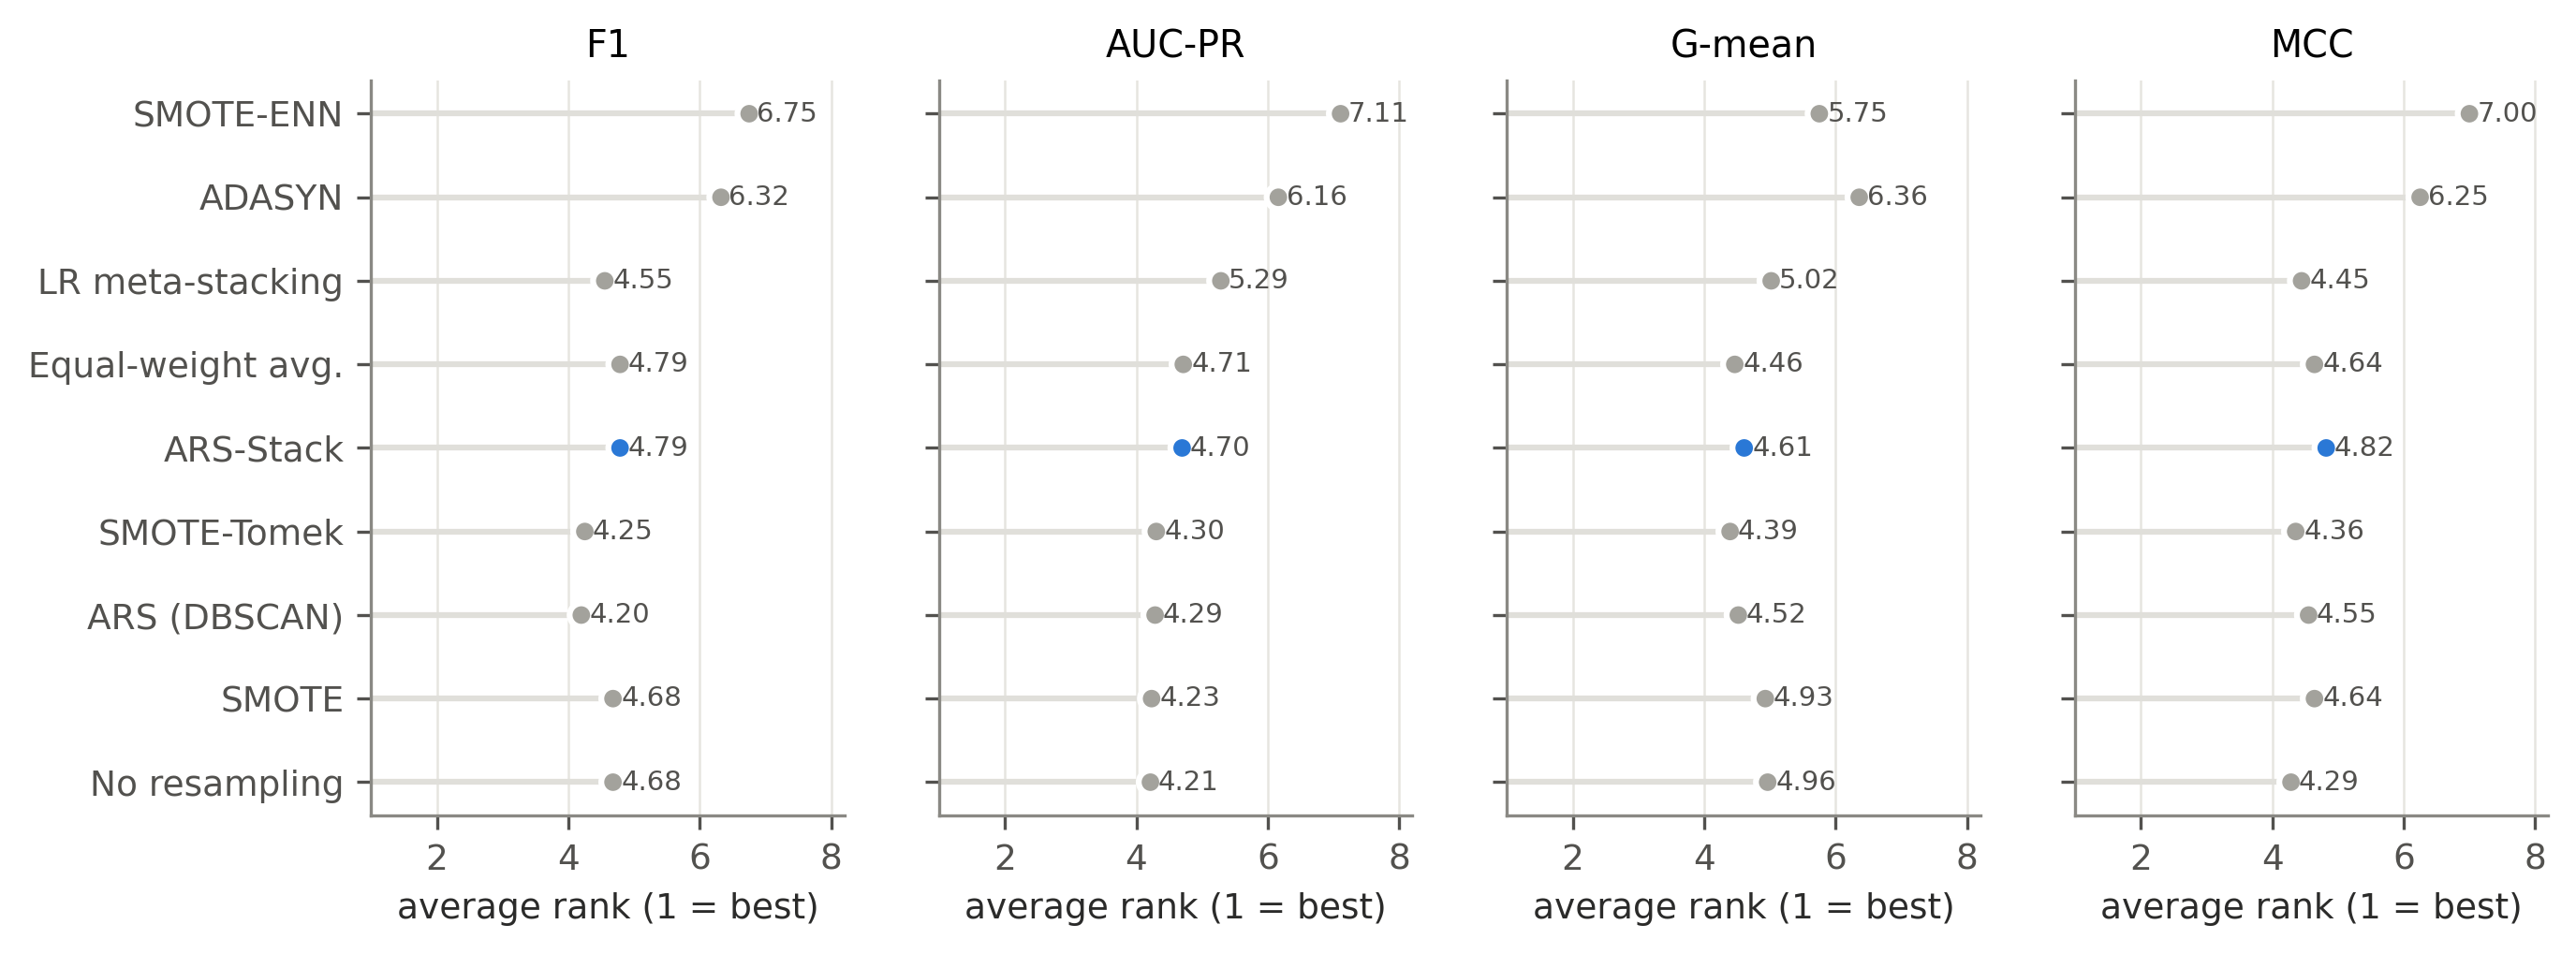
\includegraphics[width=\linewidth]{fig4_average_ranks.png}
\caption{Average rank of each variant over 28 datasets per metric (1 = best). ARS-Stack in blue.}
\label{fig:ranks}
\end{figure}

The Friedman and Iman--Davenport tests reject the hypothesis that all nine variants are equivalent for F1 ($p=1.8\times10^{-3}$), AUC-PR ($p=1.4\times10^{-4}$) and MCC ($p=5.8\times10^{-4}$), but not for G-mean ($p=0.11$) (Table~\ref{tab:ranks}). Figure~\ref{fig:ranks} shows where the differences come from. Two variants rank clearly worse than the rest on every metric: global ADASYN (mean rank 6.27) and global SMOTE-ENN (6.65). The remaining seven, including ARS-Stack, form a tight group with average ranks between 4.2 and 4.8. ARS-Stack's ranks are 4.79 (F1), 4.70 (AUC-PR), 4.61 (G-mean) and 4.82 (MCC), in the middle of this group. Mean scores tell the same story. Averaged over the 28 datasets, AUC-PR is 0.669 without resampling, 0.667 for SMOTE, 0.662 for ARS-Stack and 0.645 for SMOTE-ENN. ARS-Stack has the \emph{highest} mean MCC (0.601 versus 0.599 for SMOTE and for no resampling), but this margin of 0.003 is far below fold-to-fold variation.

\begin{table}[t]\centering\small
\caption{ARS-Stack versus each baseline across the 28 datasets: wins/ties/losses (W/T/L) of the per-dataset mean and Holm-corrected Wilcoxon signed-rank $p$-value (within each metric). Bold: $p<0.05$.}
\label{tab:xtests}
\begin{tabular}{lrrrrrrrr}
\toprule
Baseline & \multicolumn{2}{c}{F1} & \multicolumn{2}{c}{AUC-PR} & \multicolumn{2}{c}{G-mean} & \multicolumn{2}{c}{MCC} \\
 & W/T/L & $p$ & W/T/L & $p$ & W/T/L & $p$ & W/T/L & $p$ \\
\midrule
Equal-weight avg. & 11/8/9 & 1.000 & 12/3/13 & 1.000 & 8/8/12 & 1.000 & 9/8/11 & 1.000 \\
LR meta-stacking & 13/3/12 & 1.000 & 16/1/11 & 0.983 & 14/3/11 & 1.000 & 12/3/13 & 1.000 \\
ARS (DBSCAN) & 10/5/13 & 1.000 & 9/5/14 & 1.000 & 11/5/12 & 1.000 & 12/5/11 & 1.000 \\
SMOTE & 11/0/17 & 1.000 & 12/0/16 & 0.879 & 16/0/12 & 1.000 & 11/0/17 & 1.000 \\
ADASYN & 19/0/9 & 0.089 & 19/0/9 & 0.983 & 19/0/9 & 0.503 & 19/0/9 & 0.117 \\
SMOTE-Tomek & 11/0/17 & 1.000 & 14/0/14 & 0.983 & 15/0/13 & 1.000 & 11/0/17 & 1.000 \\
SMOTE-ENN & 21/0/7 & \textbf{0.041} & 22/0/6 & \textbf{0.048} & 17/0/11 & 1.000 & 22/0/6 & \textbf{0.041} \\
No resampling & 14/0/14 & 1.000 & 12/0/16 & 1.000 & 15/0/13 & 1.000 & 13/0/15 & 1.000 \\
\bottomrule
\end{tabular}
\end{table}

\begin{figure}[t]\centering
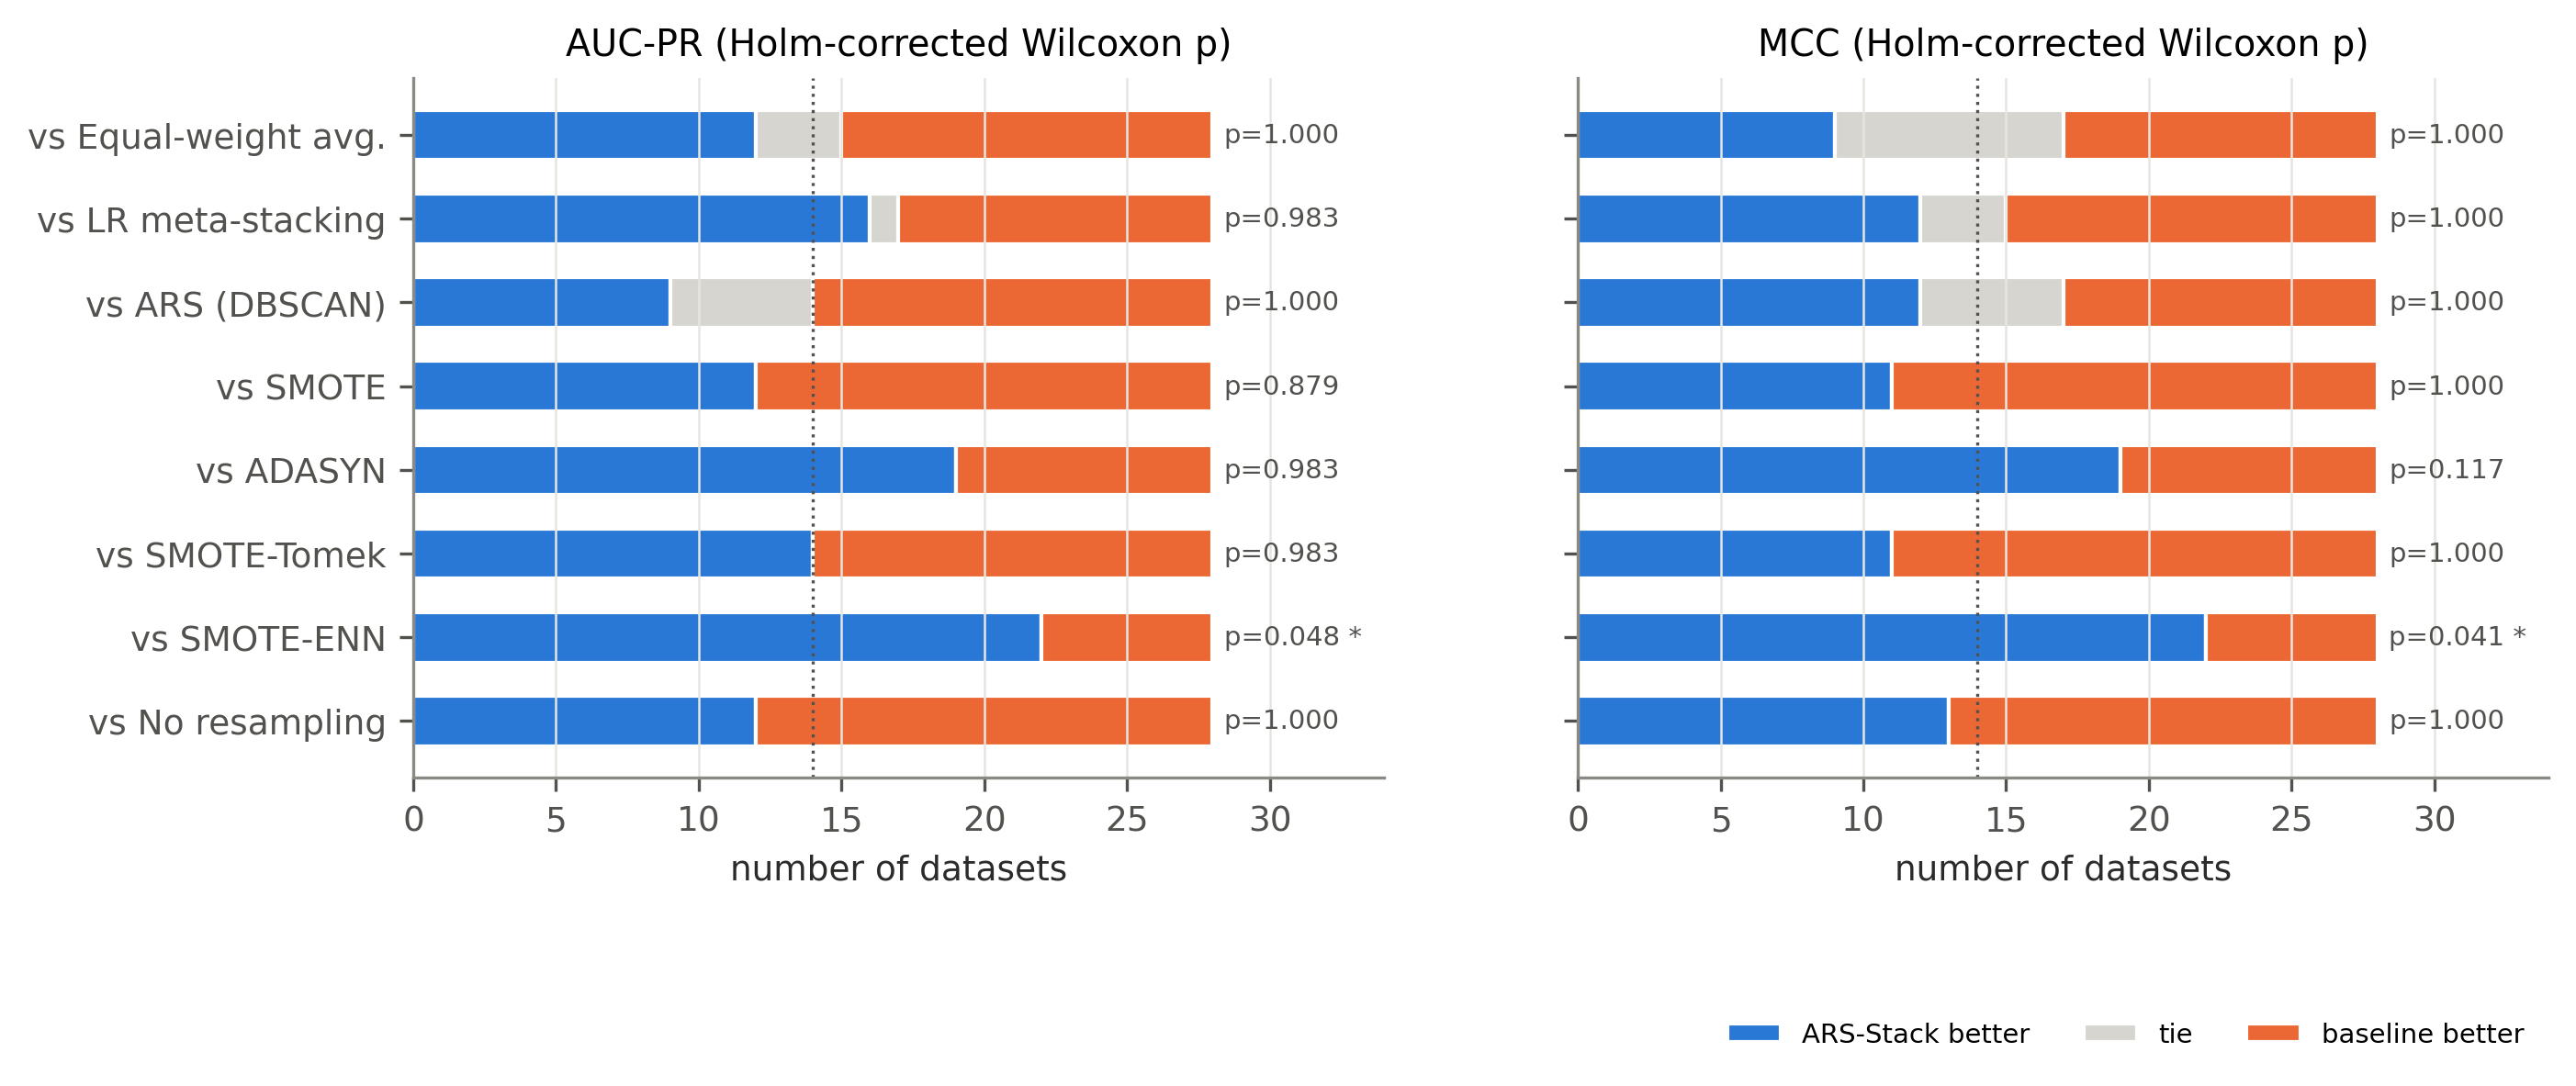
\includegraphics[width=\linewidth]{fig5_win_tie_loss.png}
\caption{Wins/ties/losses of ARS-Stack against each baseline over 28 datasets for AUC-PR and MCC, with Holm-corrected Wilcoxon $p$-values (* $p<0.05$). Dotted line: 14 datasets (an even split).}
\label{fig:wtl}
\end{figure}

The pairwise post-hoc tests in Table~\ref{tab:xtests} and Figure~\ref{fig:wtl} answer the hypotheses directly.
\begin{itemize}
  \item \textbf{H1 (adaptive vs.\ global) is supported only against SMOTE-ENN.} ARS-Stack beats global SMOTE-ENN on 22 of 28 datasets for AUC-PR and MCC and on 21 for F1 (Holm $p=0.048$, $0.041$, $0.041$). It wins 19 of 28 against global ADASYN on every metric, but this is not significant after correction ($p\ge0.089$). Against global SMOTE and SMOTE-Tomek the counts are close to even (e.g.\ 12/0/16 and 14/0/14 on AUC-PR) with $p\ge0.88$.
  \item \textbf{H2 (confidence vs.\ equal weights) is not supported.} The record is 12/3/13 on AUC-PR ($p=1.0$), with 8 exact ties on F1 and MCC.
  \item \textbf{H3 (weighted average $\ge$ meta-stacking) is supported in the weak sense.} The record is 16/1/11 on AUC-PR ($p=0.98$): the weighted average is never worse, and it is $5\times$ cheaper (Section~\ref{sec:cost}).
  \item \textbf{H4 (resampling helps) is not supported.} Against no resampling with a tuned threshold, ARS-Stack is 12/0/16 on AUC-PR and 13/0/15 on MCC ($p=1.0$).
  \item \textbf{Clustering choice is not critical.} KMeans and DBSCAN are statistically indistinguishable (9/5/14 on AUC-PR, $p=1.0$).
\end{itemize}

\subsection{Per-Dataset Analysis}

\begin{table}[t]\centering\small
\caption{Per-dataset tests: number of (dataset, metric) pairs out of $28\times4=112$ per baseline where the Holm-corrected Nadeau--Bengio corrected $t$-test is significant at $\alpha=0.05$, in favour of ARS-Stack (Win) or the baseline (Loss).}
\label{tab:sigcounts}
\begin{tabular}{llrrl}
\toprule
Baseline & Isolates & Win & Loss & Datasets \\
\midrule
Equal-weight avg. & confidence weighting & 1 & 0 & webpage \\
LR meta-stacking & weighted avg.\ vs.\ LR meta-learner & 1 & 0 & webpage \\
ARS (DBSCAN) & KMeans vs.\ DBSCAN & 0 & 0 & -- \\
SMOTE & adaptive vs.\ global SMOTE & 0 & 0 & -- \\
ADASYN & adaptive vs.\ global ADASYN & 2 & 0 & protein\_homo, webpage \\
SMOTE-Tomek & adaptive vs.\ global SMOTE-Tomek & 0 & 1 & wine\_quality \\
SMOTE-ENN & adaptive vs.\ global SMOTE-ENN & 7 & 0 & isolet, satimage, webpage \\
No resampling & resampling vs.\ none & 0 & 1 & webpage \\
\midrule
Total & & 11 & 2 & of 896 tests \\
\bottomrule
\end{tabular}
\end{table}

\begin{figure}[t]\centering
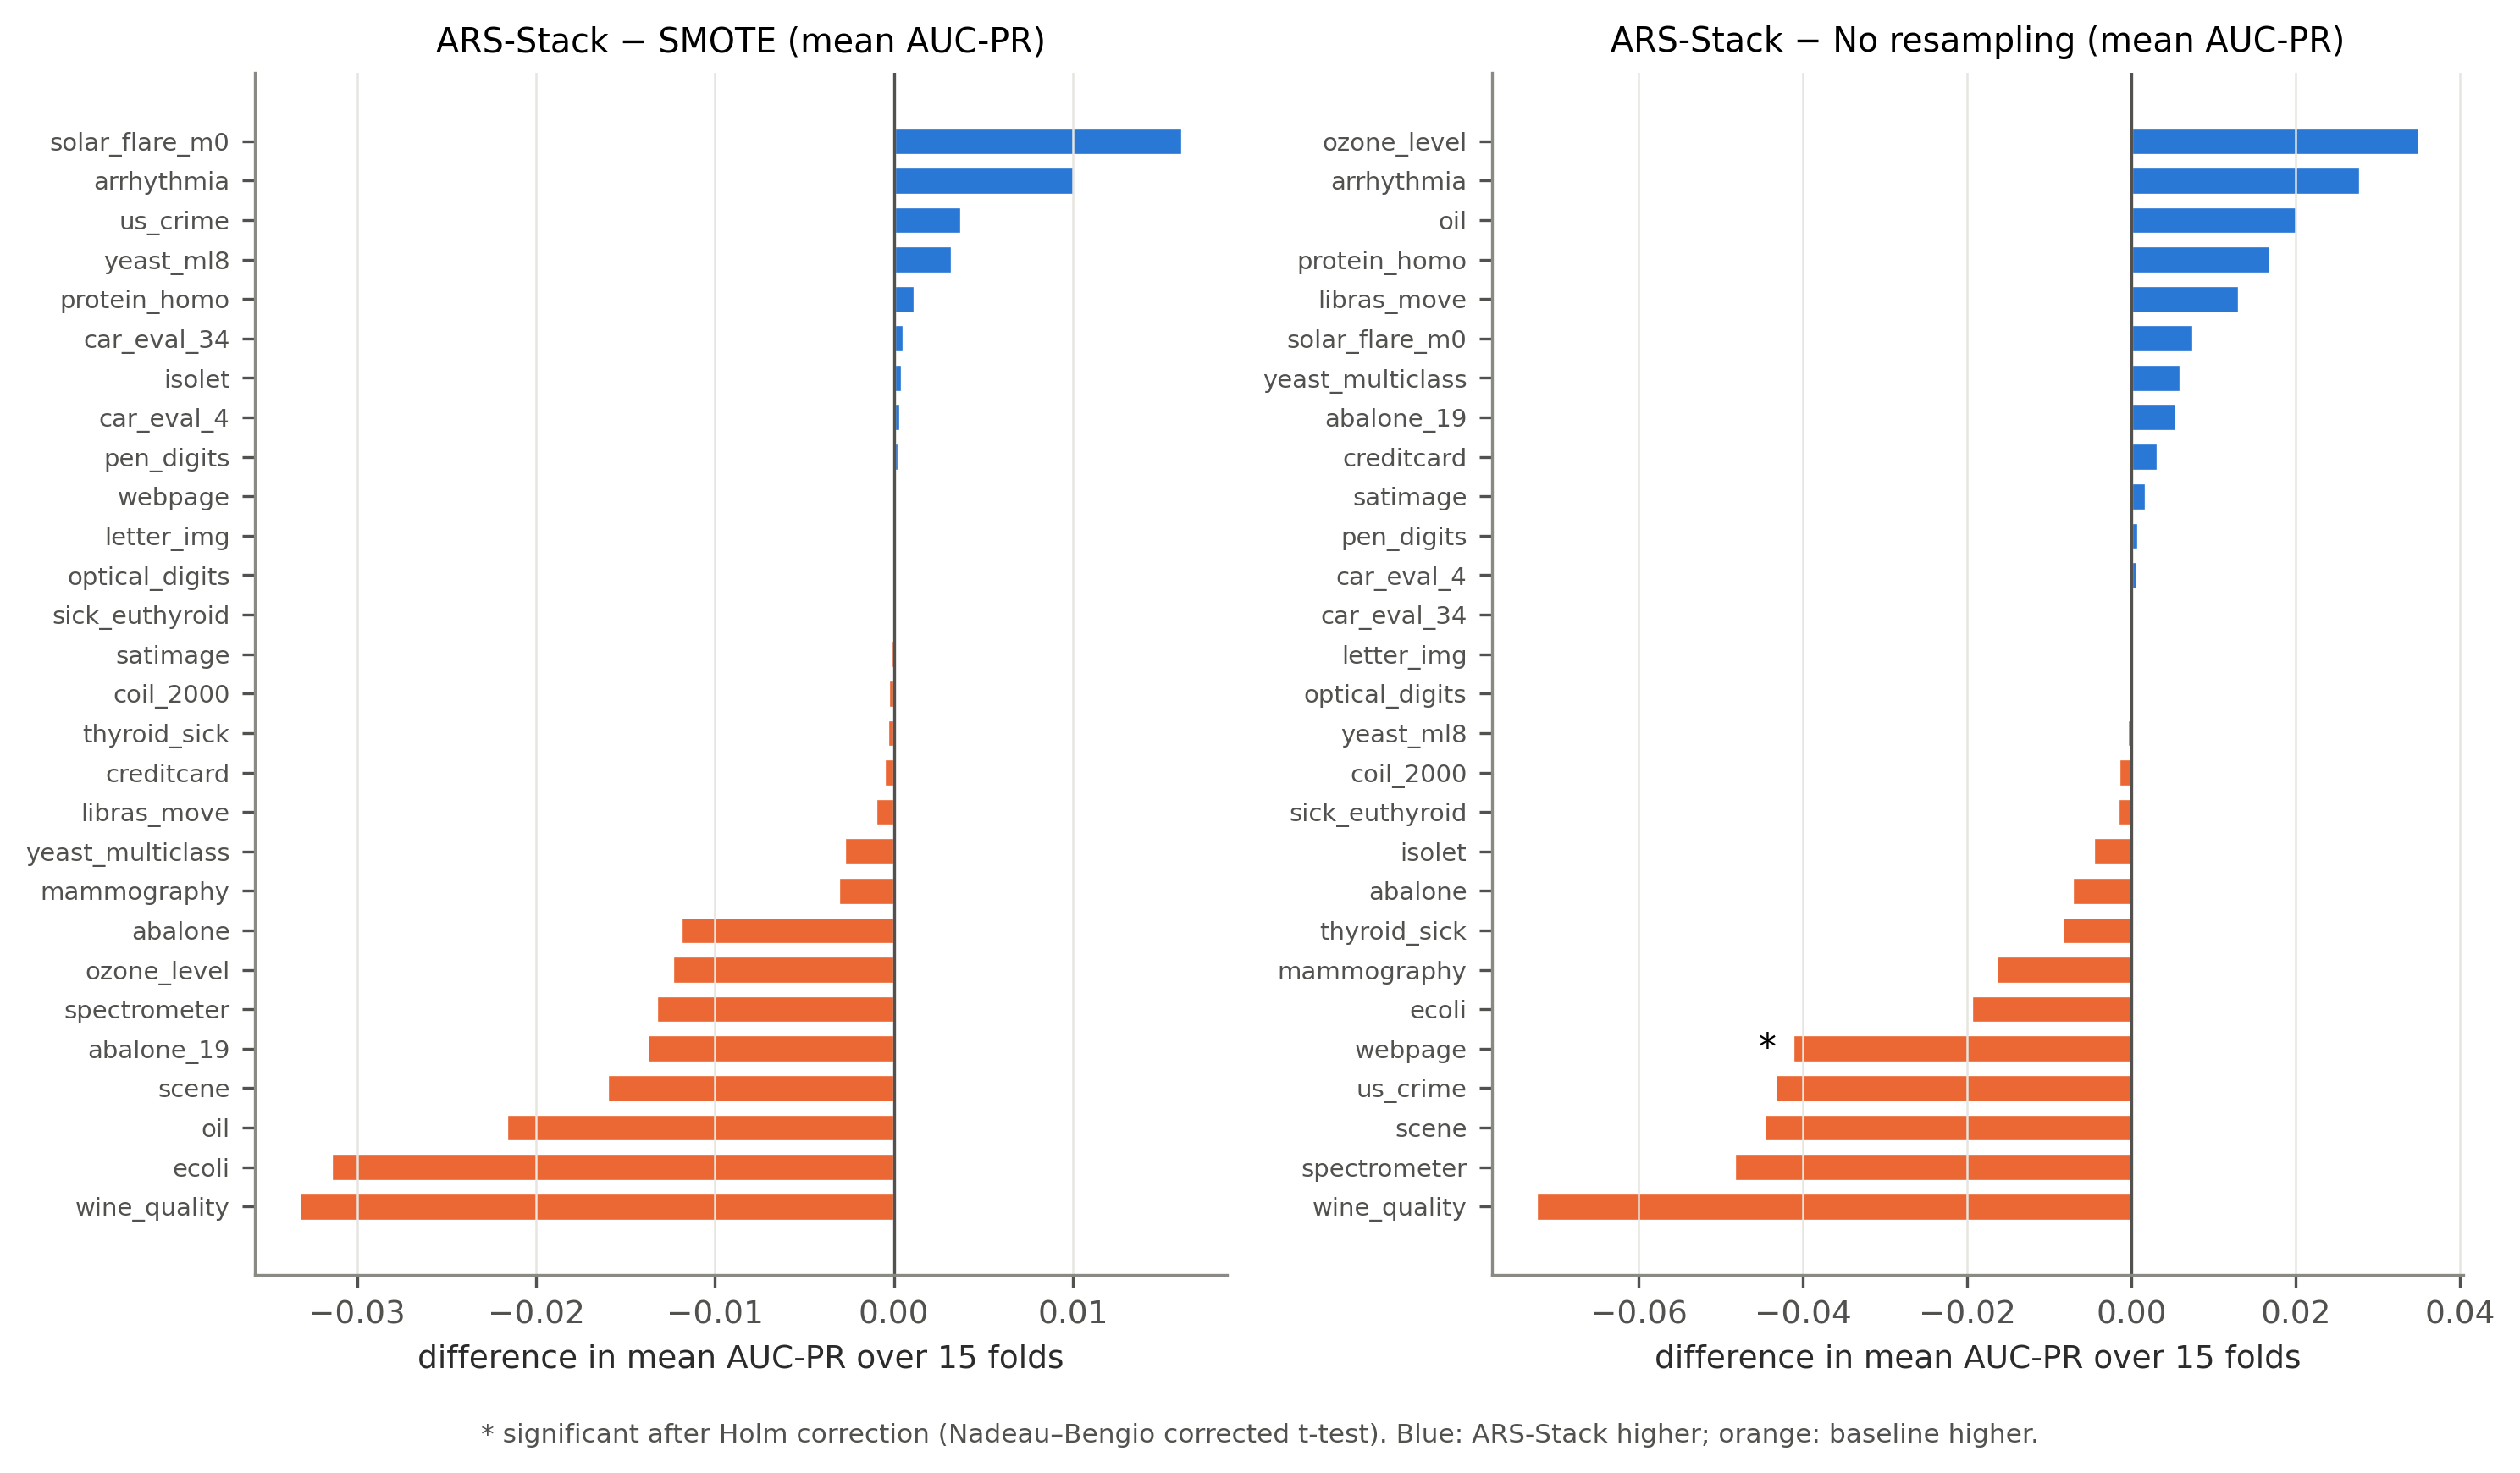
\includegraphics[width=\linewidth]{fig6_per_dataset_delta.png}
\caption{Per-dataset difference in mean AUC-PR between ARS-Stack and global SMOTE (left) and no resampling (right).}
\label{fig:delta}
\end{figure}

Within individual datasets, only 13 of the 896 Holm-corrected Nadeau--Bengio tests are significant: 11 favour ARS-Stack and 2 favour a baseline (Table~\ref{tab:sigcounts}). Seven of the 11 wins are against global SMOTE-ENN, on three high-dimensional datasets: isolet ($d=617$; AUC-PR $+0.095$), satimage ($+0.083$) and webpage ($+0.053$). On webpage, ARS-Stack is also significantly better than equal weighting, meta-stacking and global ADASYN, but significantly worse than no resampling ($-0.041$ AUC-PR). On wine\_quality, global SMOTE-Tomek is significantly better ($+0.031$).

Figure~\ref{fig:delta} shows the per-dataset differences against SMOTE and against no resampling. Against SMOTE, the median difference is $-0.0002$ and the range is $[-0.033,+0.016]$, with ARS-Stack ahead on 12 of 28 datasets. The largest losses (wine\_quality, ecoli, oil) occur where the rule sends all or most minority points to a cleaning resampler, which never happens under global SMOTE. Against no resampling the differences are larger in both directions, from $-0.073$ on wine\_quality to $+0.035$ on ozone\_level. This is consistent with the general finding that whether resampling helps depends on the dataset \cite{kovacs2019empirical}.

\subsection{Core Datasets}

\begin{table}[t]\centering\small
\caption{Core datasets: mean $\pm$ standard deviation over 15 folds (5-fold CV $\times$ 3 repeats). Yeast metrics are macro-averaged. Best mean per column in bold.}
\label{tab:core}
\setlength{\tabcolsep}{3pt}\footnotesize
\begin{tabular}{lrrrrrr}
\toprule
& \multicolumn{2}{c}{Credit card (IR 600)} & \multicolumn{2}{c}{Mammography (IR 30)} & \multicolumn{2}{c}{Yeast, 10 classes} \\
Variant & AUC-PR & MCC & AUC-PR & MCC & AUC-PR & MCC \\
\midrule
\textbf{ARS-Stack} & 0.843$\pm$0.027 & 0.848$\pm$0.022 & 0.763$\pm$0.046 & 0.693$\pm$0.049 & 0.597$\pm$0.041 & 0.447$\pm$0.032 \\
Equal-weight avg. & 0.842$\pm$0.025 & 0.846$\pm$0.020 & 0.763$\pm$0.046 & 0.688$\pm$0.051 & 0.597$\pm$0.041 & 0.448$\pm$0.032 \\
LR meta-stacking & 0.843$\pm$0.026 & 0.849$\pm$0.022 & 0.760$\pm$0.046 & 0.696$\pm$0.049 & 0.579$\pm$0.062 & \textbf{0.471$\pm$0.025} \\
ARS (DBSCAN) & \textbf{0.844$\pm$0.027} & 0.849$\pm$0.026 & 0.750$\pm$0.043 & 0.676$\pm$0.046 & \textbf{0.601$\pm$0.038} & 0.450$\pm$0.032 \\
SMOTE & 0.844$\pm$0.028 & 0.848$\pm$0.026 & 0.766$\pm$0.047 & 0.693$\pm$0.041 & 0.599$\pm$0.038 & 0.447$\pm$0.034 \\
ADASYN & 0.836$\pm$0.032 & 0.845$\pm$0.021 & 0.739$\pm$0.047 & 0.694$\pm$0.048 & 0.586$\pm$0.038 & 0.438$\pm$0.033 \\
SMOTE-Tomek & 0.844$\pm$0.028 & 0.848$\pm$0.026 & 0.767$\pm$0.047 & 0.703$\pm$0.033 & 0.599$\pm$0.047 & 0.452$\pm$0.035 \\
SMOTE-ENN & 0.830$\pm$0.032 & 0.830$\pm$0.031 & 0.722$\pm$0.058 & 0.654$\pm$0.040 & 0.566$\pm$0.047 & 0.388$\pm$0.032 \\
No resampling & 0.840$\pm$0.027 & \textbf{0.855$\pm$0.023} & \textbf{0.780$\pm$0.042} & \textbf{0.703$\pm$0.050} & 0.591$\pm$0.057 & 0.444$\pm$0.041 \\
\bottomrule
\end{tabular}
\end{table}

\begin{figure}[t]\centering
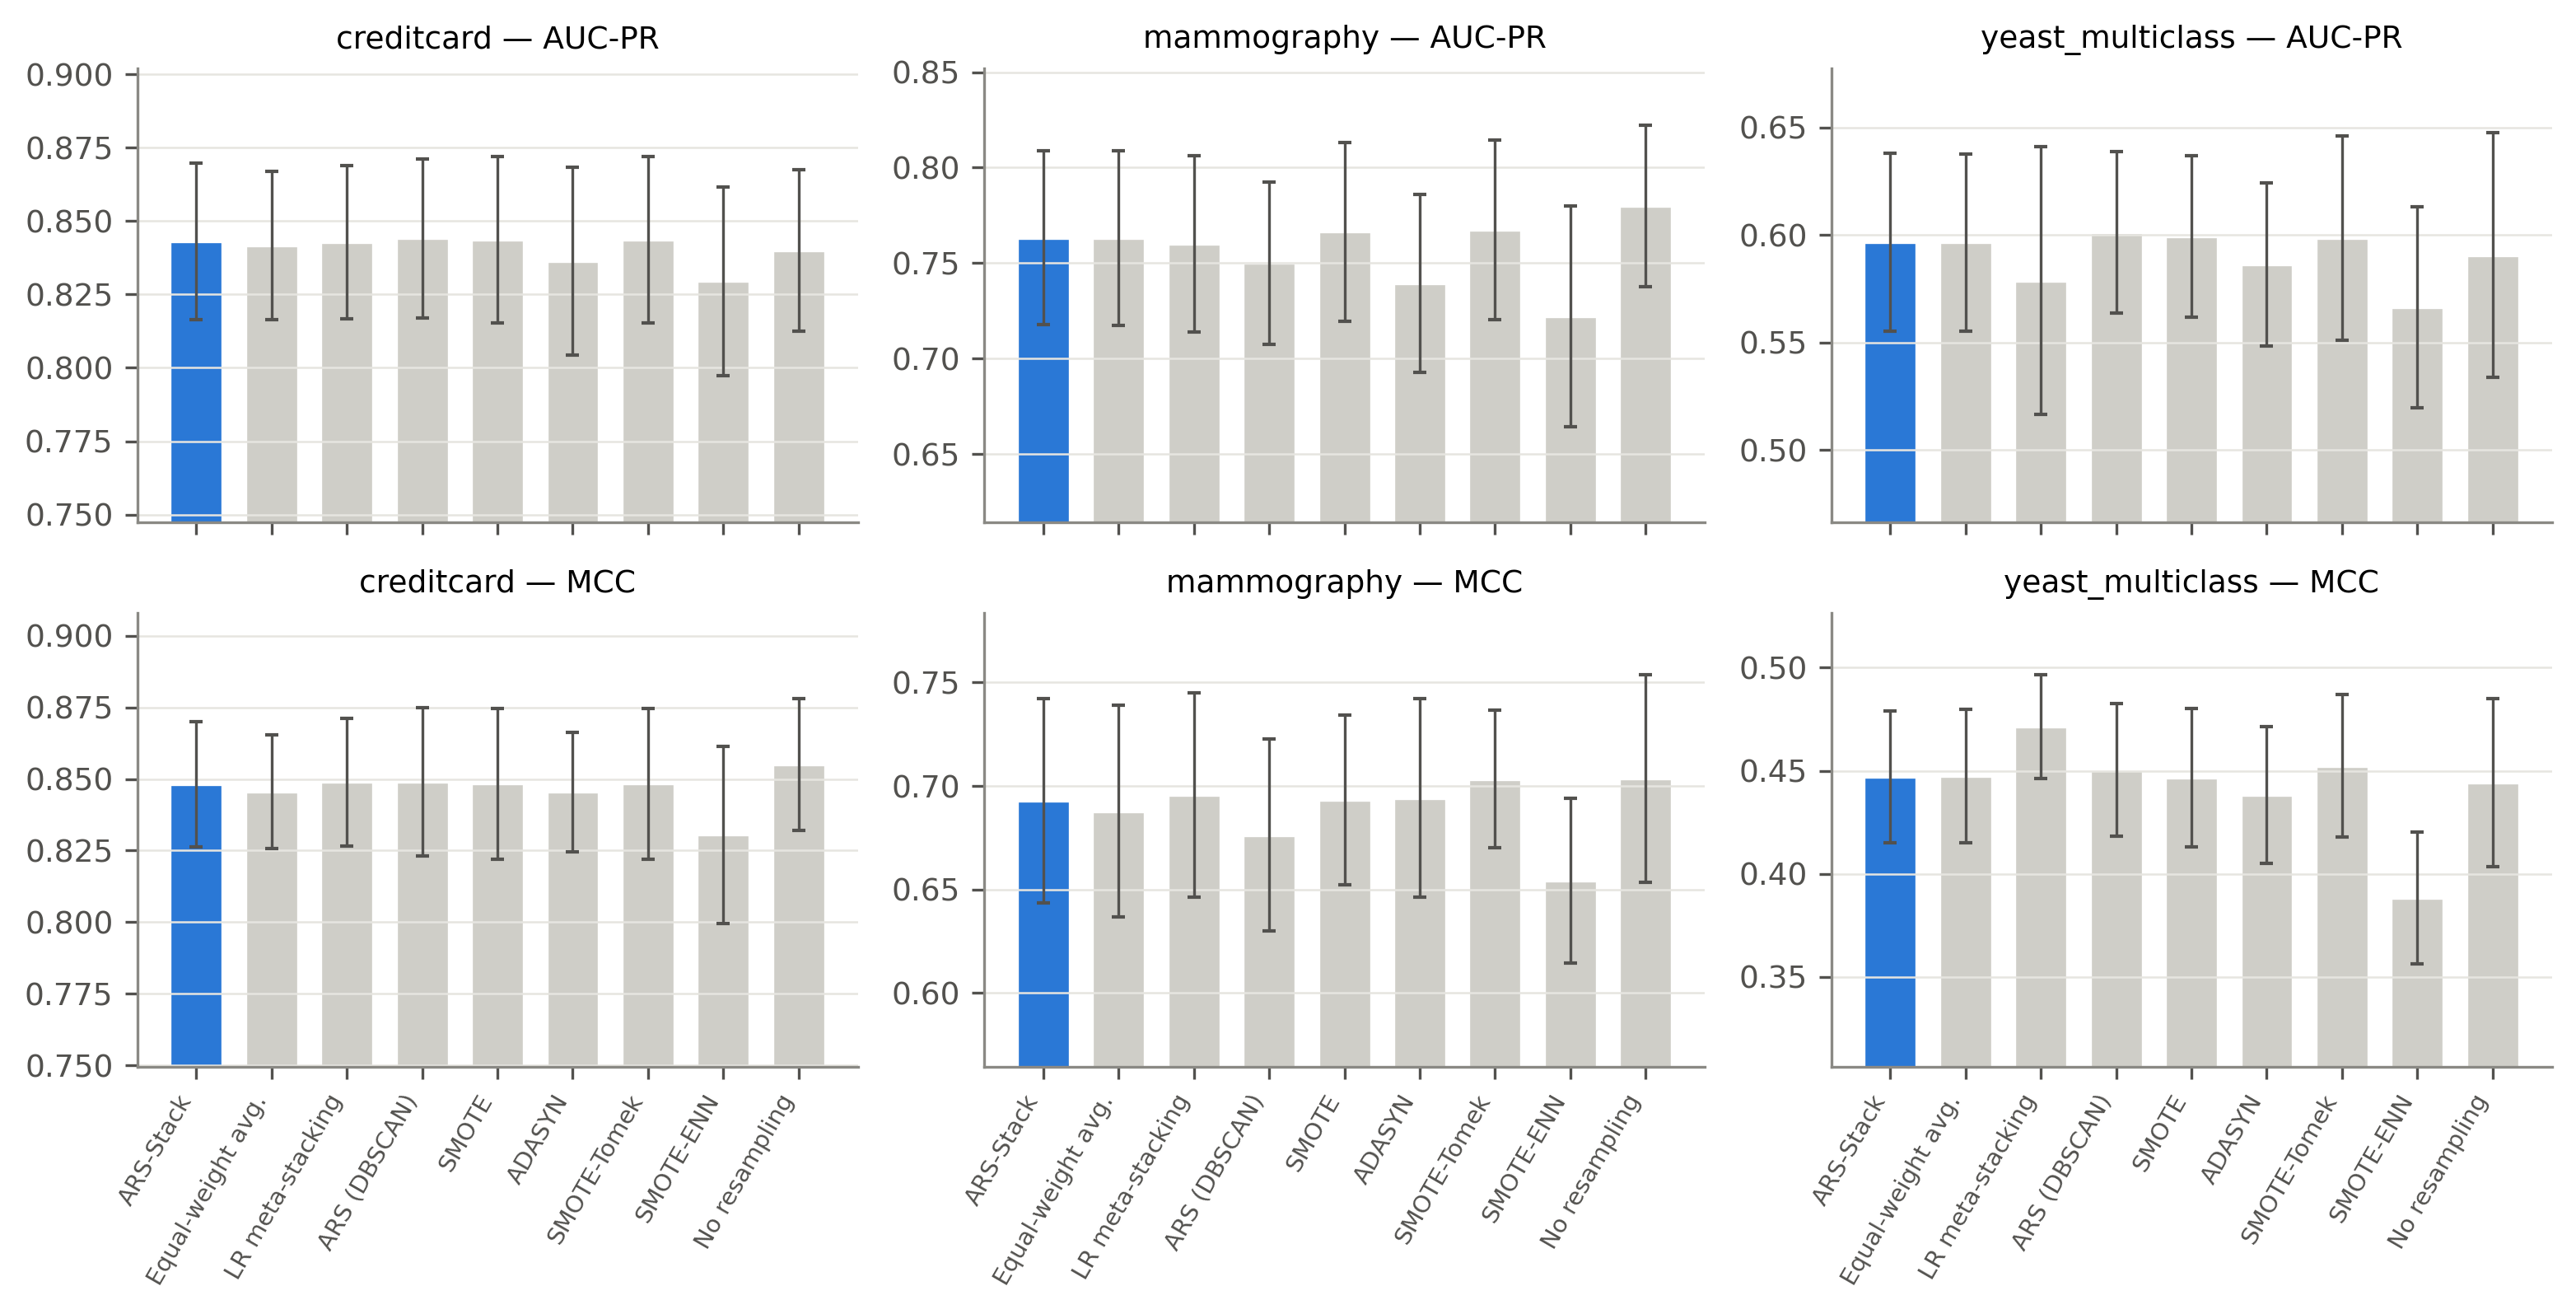
\includegraphics[width=\linewidth]{fig11_core_datasets.png}
\caption{Core datasets: mean $\pm$ standard deviation over 15 folds for AUC-PR (top) and MCC (bottom). ARS-Stack in blue.}
\label{fig:core}
\end{figure}

On credit-card fraud, every variant except SMOTE-ENN and ADASYN reaches an AUC-PR of 0.840--0.844 and an MCC of 0.846--0.855 (Table~\ref{tab:core}, Figure~\ref{fig:core}). ARS-Stack scores $0.843\pm0.027$ AUC-PR and $0.848\pm0.022$ MCC; the fold standard deviation is about ten times the spread between variants. On mammography, no resampling is best on AUC-PR ($0.780$ versus $0.763$ for ARS-Stack), while ARS-Stack, SMOTE and SMOTE-Tomek tie on MCC at 0.69--0.70. On multiclass yeast, ARS-Stack, equal weighting, ARS (DBSCAN), SMOTE and SMOTE-Tomek are within 0.005 macro-AUC-PR (0.597--0.601). Meta-stacking has the best macro-MCC (0.471 versus 0.447) but a lower macro-AUC-PR (0.579). Table~\ref{tab:single} reports the single fixed-split runs and the reproduced SMOTE-based baselines. On a single split, ARS-Stack and the same ensemble with global SMOTE are identical to three decimals on credit card, because the selector chose SMOTE for both minority clusters. On mammography, the single split favours global SMOTE (F1 0.609 versus 0.541), but the CV results show that this split is not representative ($0.693\pm0.049$ versus $0.693\pm0.041$ MCC). This illustrates why single-split comparisons, common in the literature, are unreliable.

\begin{table}[t]\centering\small
\caption{Single fixed stratified split (20\% test; 10\% of the remainder for validation; seed 42): ARS-Stack, the same ensemble with global SMOTE, and reproduced SMOTE-based baselines (RF, XGBoost, two-learner LR stacking). One split only; see Table~\ref{tab:core} for the CV estimates.}
\label{tab:single}
\begin{tabular}{llrrrr}
\toprule
Dataset & Model & F1 & AUC-PR & G-mean & MCC \\
\midrule
creditcard & ARS-Stack (adaptive) & 0.817 & 0.820 & 0.840 & 0.827 \\
creditcard & Our ensemble + global SMOTE & 0.817 & 0.821 & 0.840 & 0.827 \\
creditcard & Random Forest + SMOTE & 0.832 & 0.821 & 0.871 & 0.836 \\
creditcard & XGBoost + SMOTE & 0.775 & 0.818 & 0.894 & 0.775 \\
creditcard & LR stacking (RF+XGB) + SMOTE & 0.815 & 0.823 & 0.888 & 0.815 \\
\midrule
mammography & ARS-Stack (adaptive) & 0.541 & 0.620 & 0.669 & 0.540 \\
mammography & Our ensemble + global SMOTE & 0.609 & 0.632 & 0.738 & 0.601 \\
mammography & Random Forest + SMOTE & 0.615 & 0.606 & 0.787 & 0.602 \\
mammography & XGBoost + SMOTE & 0.630 & 0.639 & 0.810 & 0.618 \\
mammography & LR stacking (RF+XGB) + SMOTE & 0.647 & 0.636 & 0.800 & 0.635 \\
\midrule
yeast\_multiclass & ARS-Stack (adaptive) & 0.502 & 0.657 & 0.692 & 0.483 \\
yeast\_multiclass & Our ensemble + global SMOTE & 0.514 & 0.668 & 0.701 & 0.533 \\
\bottomrule
\end{tabular}
\end{table}

Published credit-card results often report higher F1 or AUC-PR than ours. They are not comparable. Those studies usually keep the 1{,}081 duplicate rows (which can leak between train and test splits), evaluate a single split, and sometimes tune on the test set. Our numbers are cross-validated, deduplicated and leakage-free.

\subsection{What the Selector Does}

\begin{figure}[t]\centering
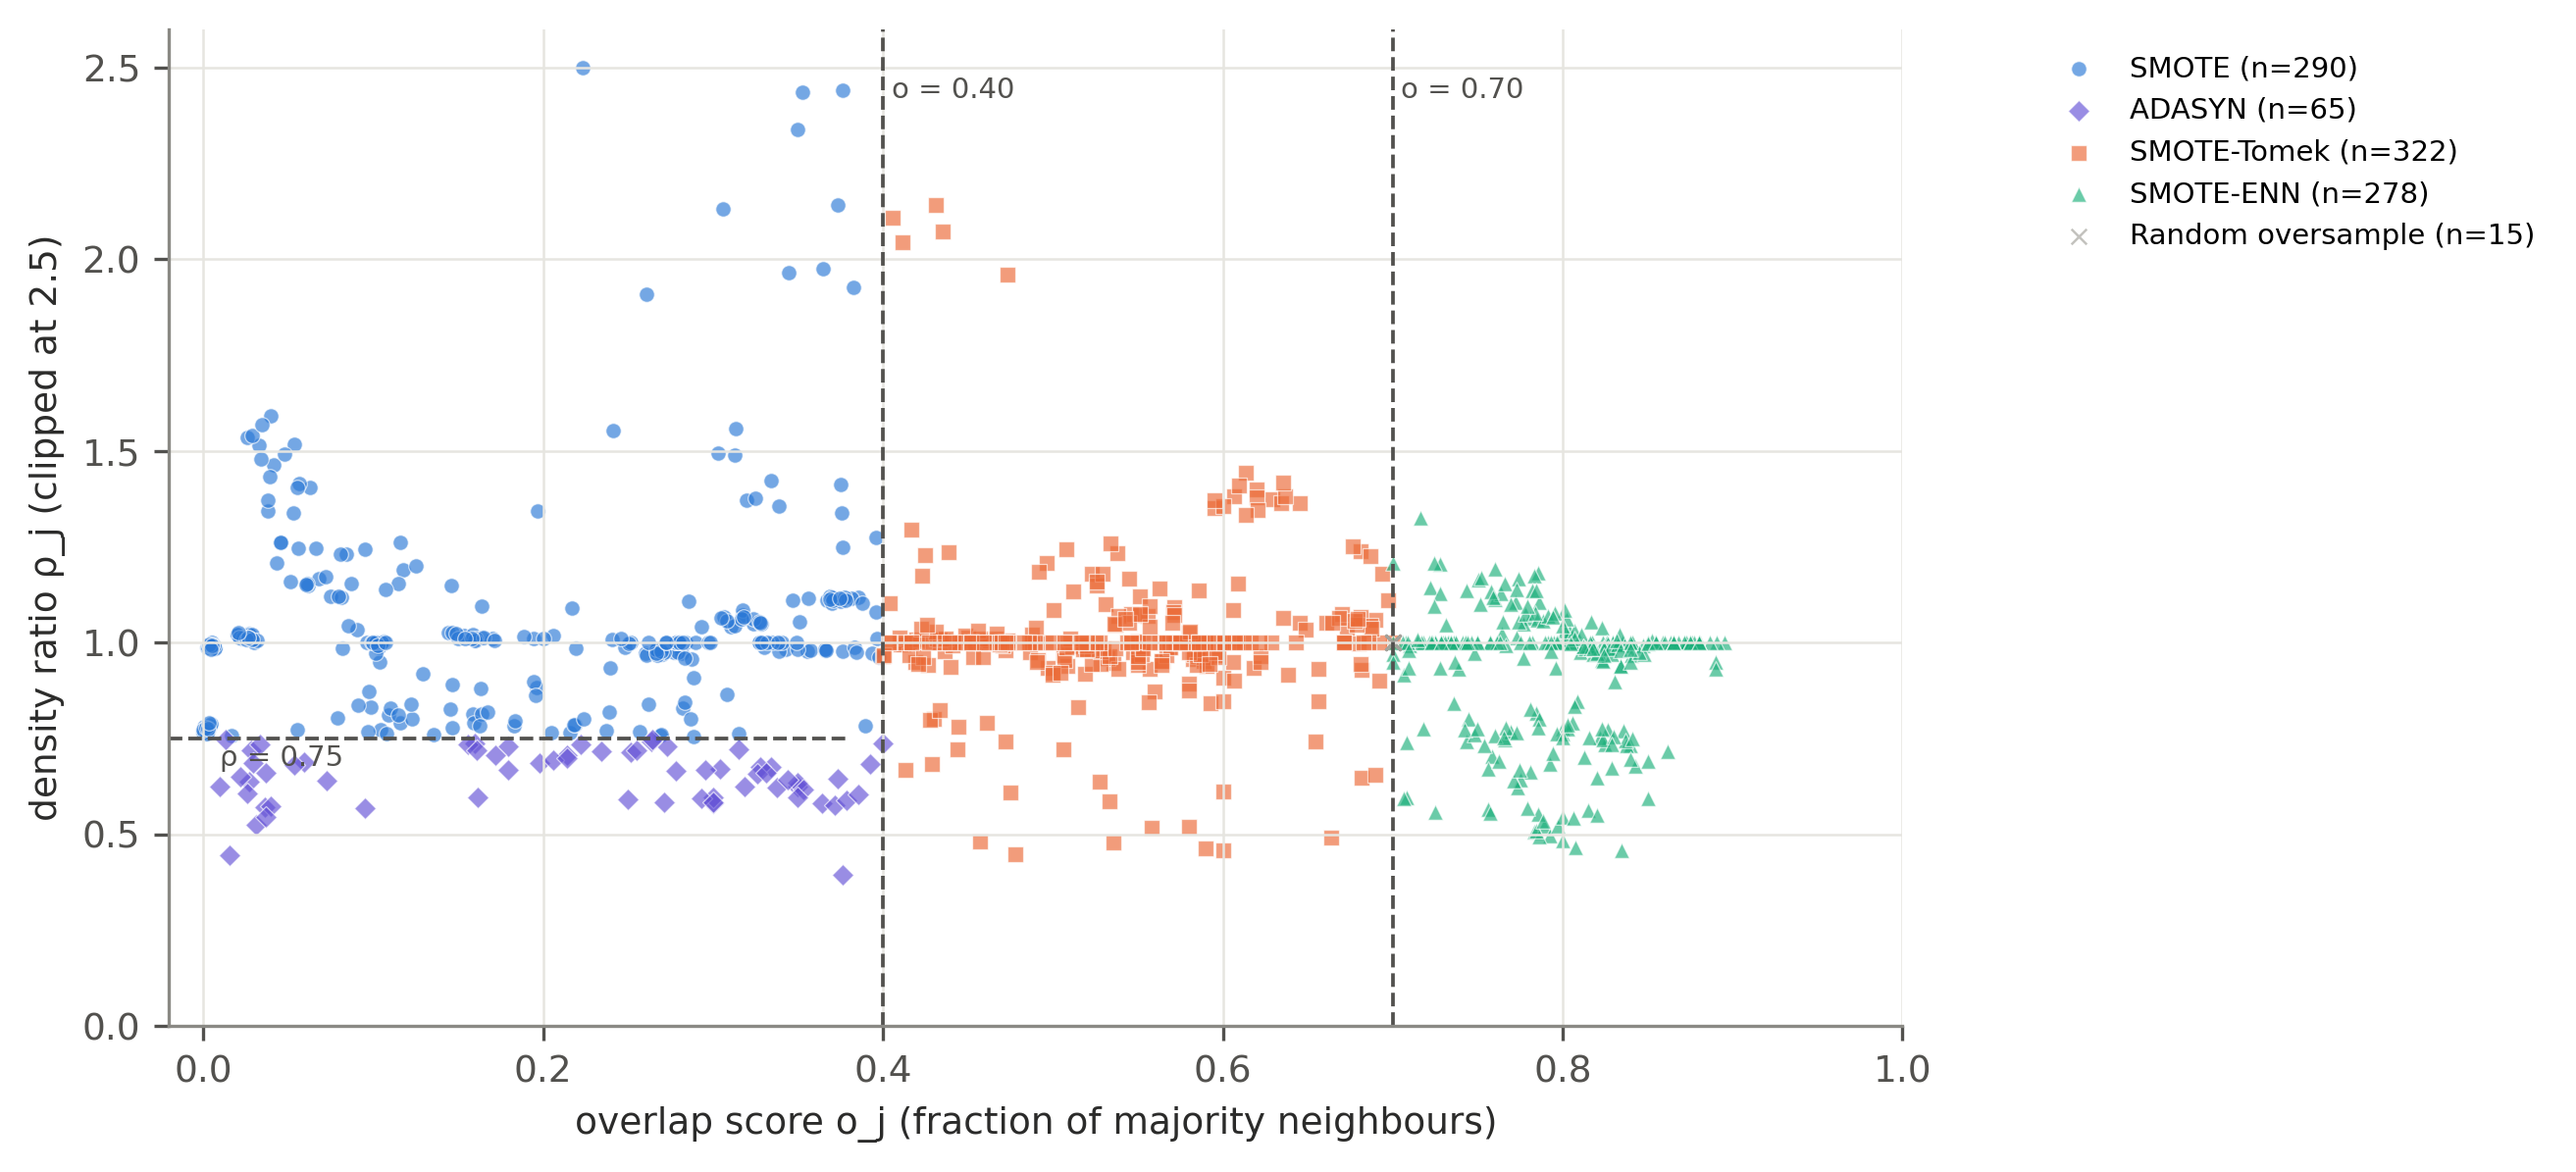
\includegraphics[width=0.9\linewidth]{fig7_cluster_space.png}
\caption{All 970 minority clusters formed by ARS-Stack (28 datasets $\times$ 15 folds) in the (overlap, density-ratio) plane, coloured by the selected resampler; dashed lines are the fixed thresholds of Eq.~\ref{eq:rule}.}
\label{fig:clusters}
\end{figure}

\begin{figure}[t]\centering
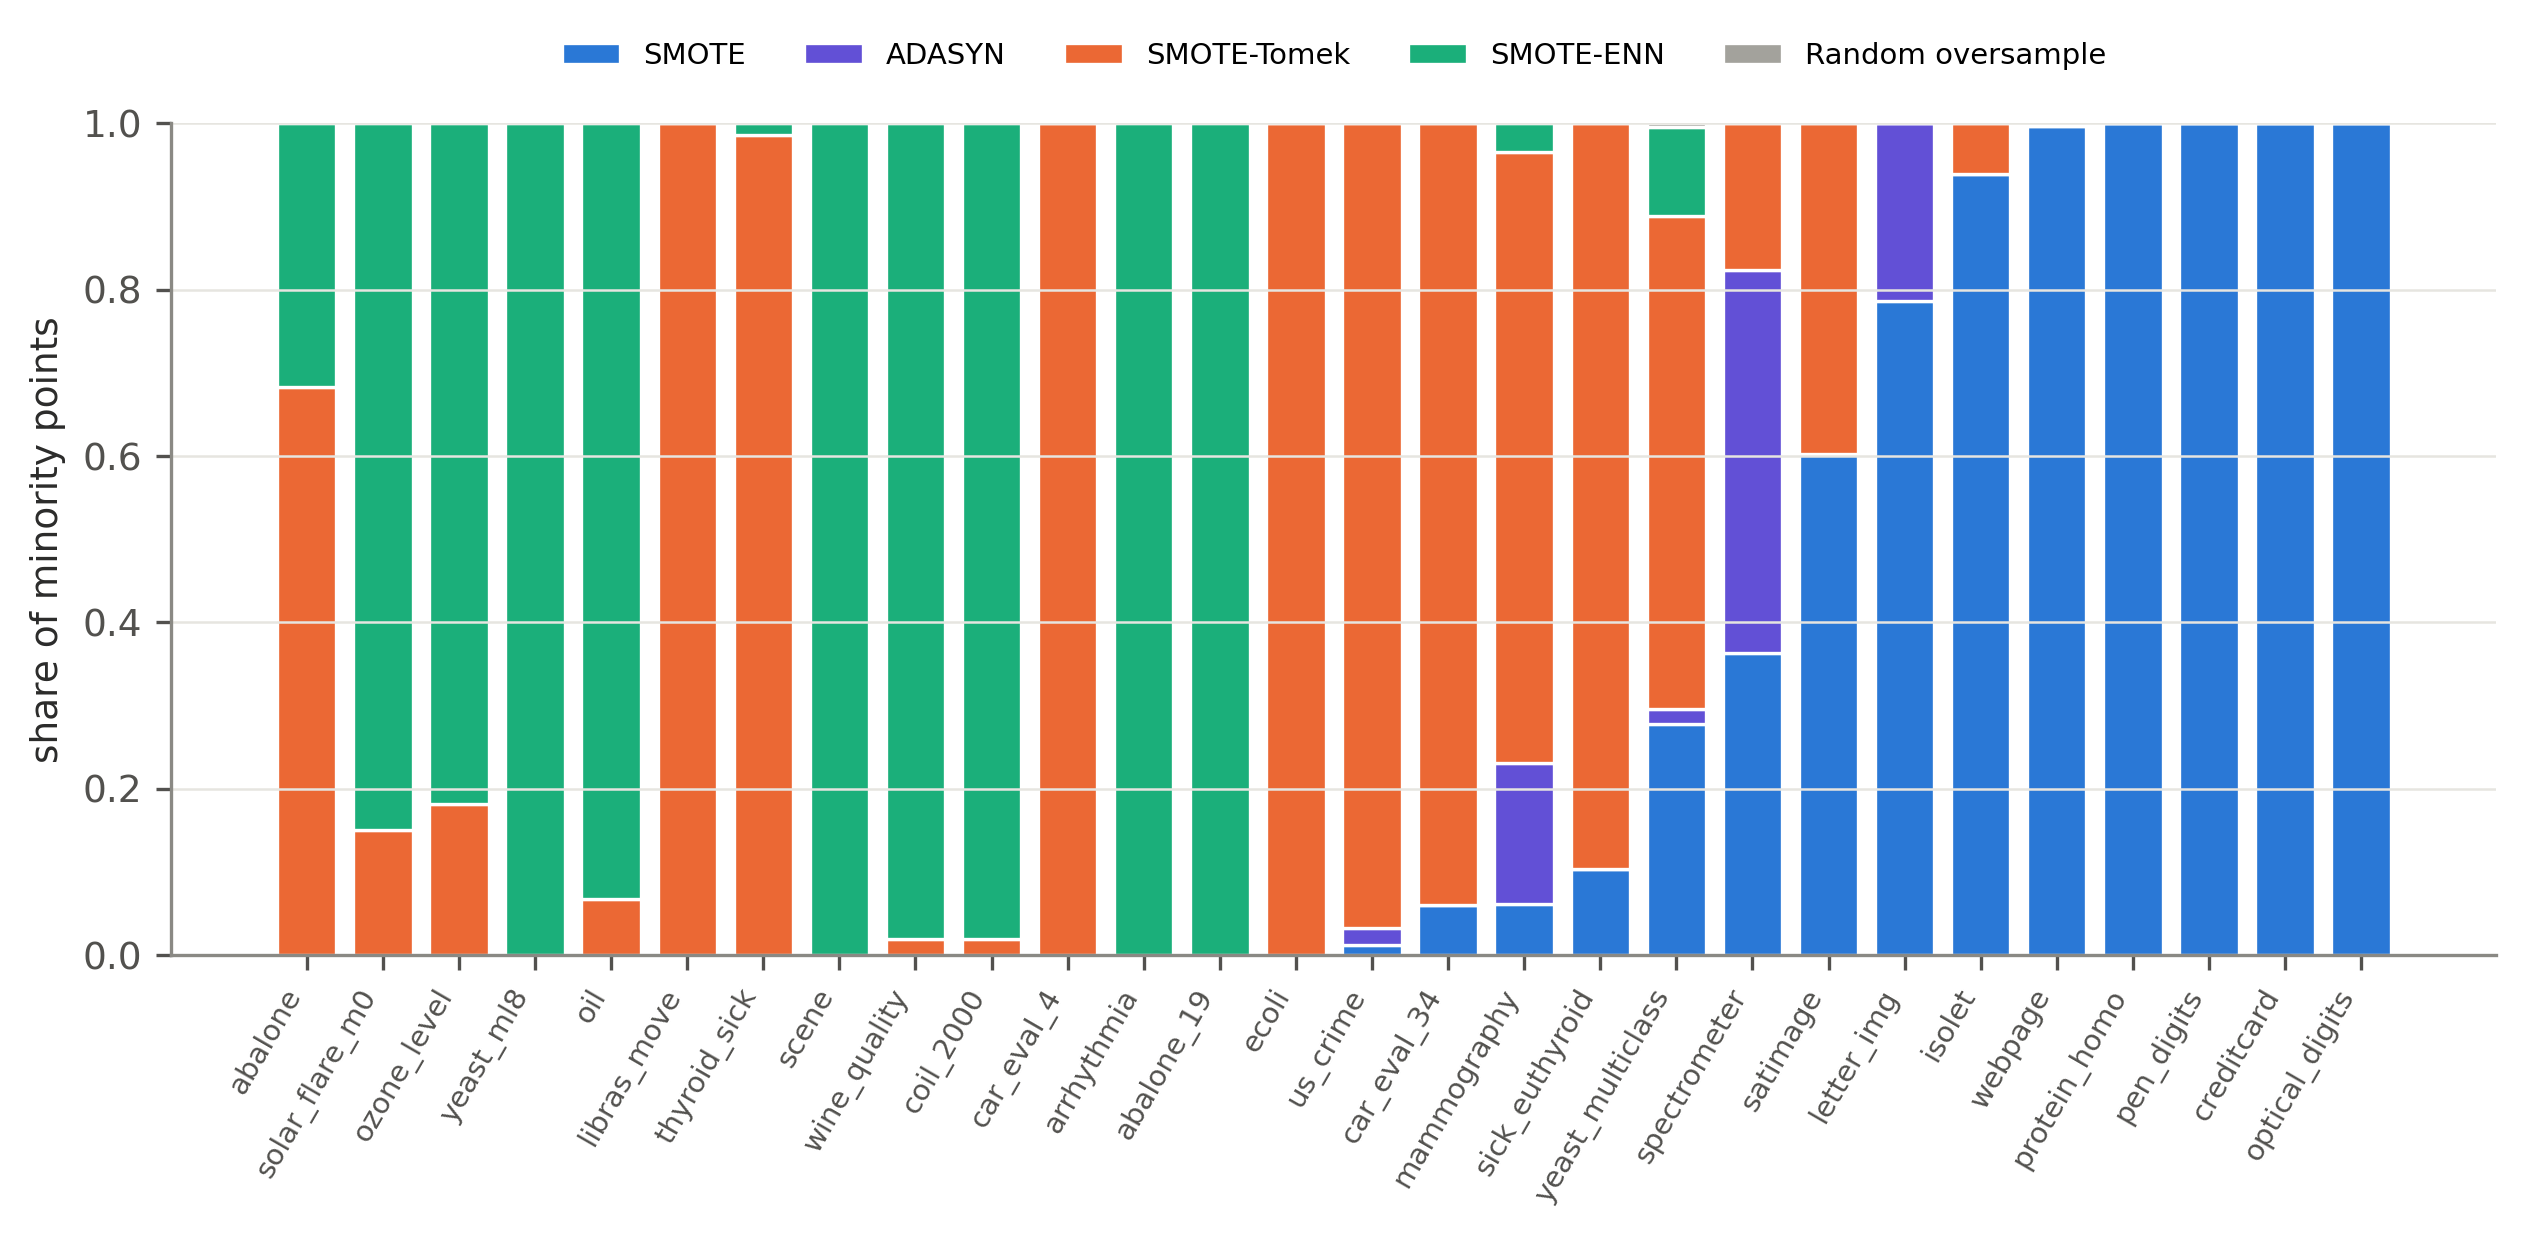
\includegraphics[width=\linewidth]{fig8_resampler_share.png}
\caption{Share of minority points assigned to each resampler, per dataset (ARS-Stack, all folds).}
\label{fig:share}
\end{figure}

Over all folds, ARS-Stack formed 970 minority clusters, an average of 1.8 per class and fold (Figure~\ref{fig:clusters}). They were assigned to SMOTE-Tomek (322), SMOTE (290), SMOTE-ENN (278), ADASYN (65) and random oversampling (15). Weighted by points, 60.3\% of minority samples were handled by SMOTE, 22.4\% by SMOTE-Tomek, 15.1\% by SMOTE-ENN and 2.2\% by ADASYN. The selector is therefore genuinely active, with all four resamplers used. Figure~\ref{fig:share} shows, however, that the choice is often uniform \emph{within} a dataset: on 11 of 28 datasets every minority point received the same resampler. This happens because silhouette-selected KMeans usually returns $k=2$ and both clusters fall on the same side of the thresholds, or because small minority classes are treated as one cluster. On those datasets ARS-Stack is a \emph{local} version of one global method, and its adaptivity cannot help.

\subsection{Why Adaptive Selection Behaves Like SMOTE}

\begin{table}[t]\centering\small
\caption{Percentage of majority-class training rows removed by the cleaning step, over all $28\times15$ folds. ARS-Stack cleans only the local majority context of each cluster.}
\label{tab:removed}
\begin{tabular}{lrrrr}
\toprule
Variant & Median & Mean & 90th pct. & Max \\
\midrule
ARS-Stack & 0.0 & 3.4 & 10.3 & 36.7 \\
SMOTE-Tomek & 0.0 & 0.7 & 0.5 & 17.5 \\
SMOTE-ENN & 13.9 & 19.5 & 48.4 & 92.6 \\
\bottomrule
\end{tabular}
\end{table}

The key mechanistic finding is in Table~\ref{tab:removed}. Global SMOTE-ENN removes a median of 13.9\% of majority training rows, 48.4\% at the 90th percentile and up to 92.6\%. On overlapping datasets this destroys much of the majority class and explains its poor ranks. Global SMOTE-Tomek removes almost nothing (mean 0.7\%), so it behaves like SMOTE, which is why the SMOTE and SMOTE-Tomek columns in Figure~\ref{fig:delta} and Table~\ref{tab:full_auc_pr} are nearly identical. ARS-Stack applies ENN only inside the local majority context of high-overlap clusters, and removes a median of 0\% and a mean of 3.4\% of majority rows. Even when the selector picks SMOTE-ENN for 100\% of the minority points, as on yeast\_ml8, arrhythmia and scene, ARS-Stack removes 10--21\% of the majority rows against 42--66\% for global SMOTE-ENN. ARS-Stack therefore keeps the noise-robustness intent of cleaning without its data loss. This is exactly why it significantly beats global SMOTE-ENN. It is also why it cannot be expected to differ much from SMOTE.

\subsection{Confidence Weights are Near-Uniform}

\begin{figure}[t]\centering
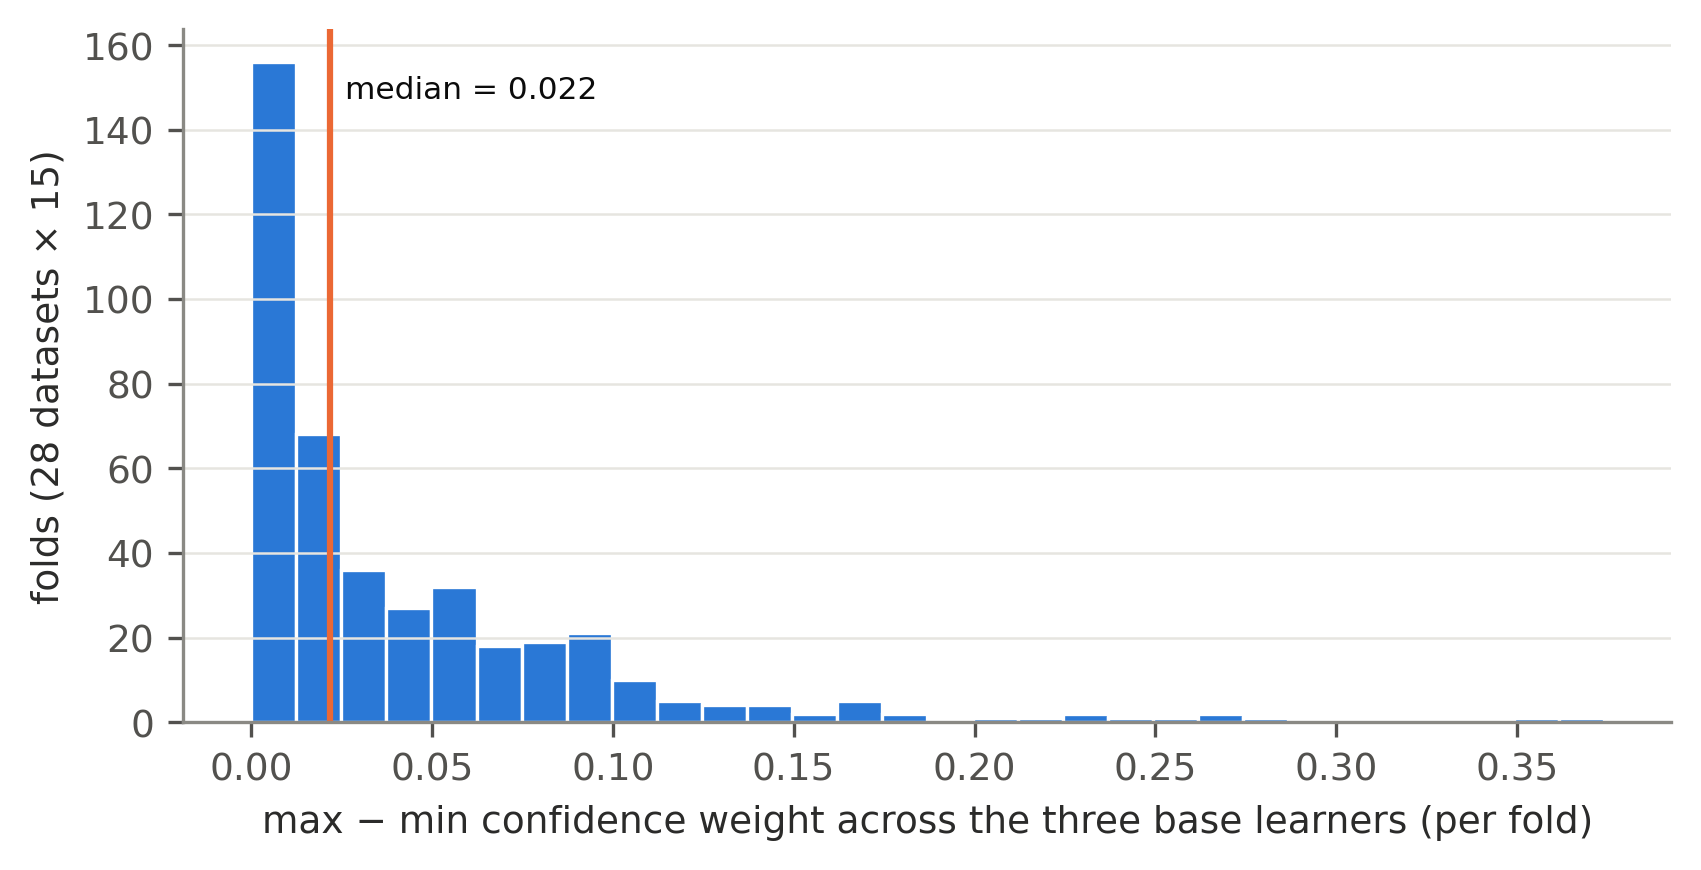
\includegraphics[width=0.72\linewidth]{fig9_weight_spread.png}
\caption{Spread (max $-$ min) of the three confidence weights in each of the 420 ARS-Stack folds.}
\label{fig:weights}
\end{figure}

Hypothesis H2 fails for a simple reason (Figure~\ref{fig:weights}). Random Forest, XGBoost and LightGBM reach similar validation AUC-PR, so the normalised weights stay close to $1/3$. The median spread between the largest and smallest weight is 0.022, the 90th percentile is 0.100, and no learner ever received more than 0.571. A weighted average with near-equal weights is almost an equal-weight average, hence the 8 exact ties. Weights that are proportional to AUC-PR are too flat to matter when the learners are all strong. A sharper mapping (e.g.\ a softmax with temperature) might, but would need an extra hyperparameter tuned without test data.

\subsection{Does the Benefit Depend on Dataset Properties?}

\begin{figure}[t]\centering
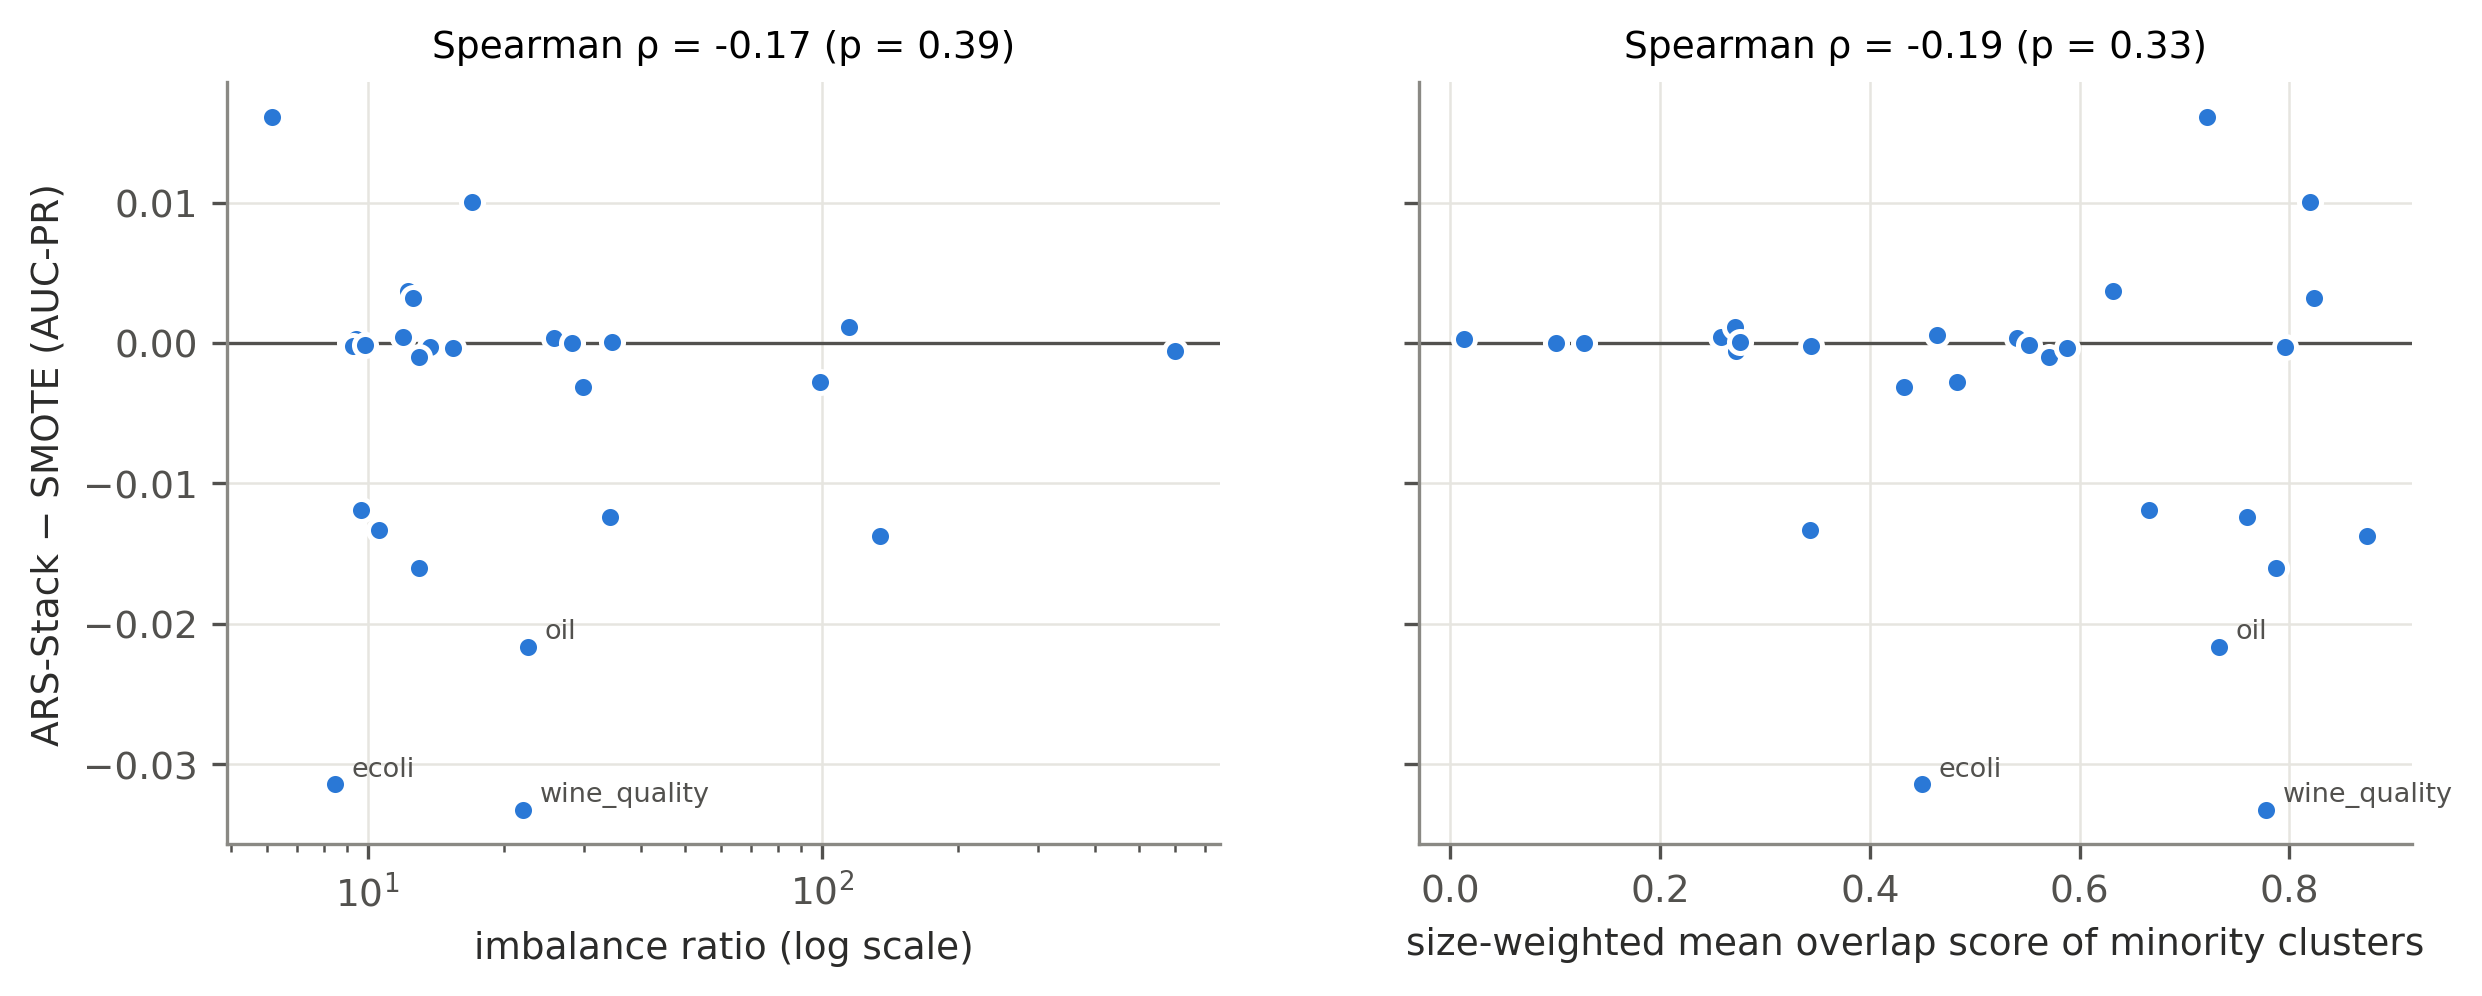
\includegraphics[width=0.95\linewidth]{fig12_delta_vs_properties.png}
\caption{ARS-Stack $-$ SMOTE (AUC-PR) against imbalance ratio (left) and against the size-weighted mean overlap of the minority clusters (right).}
\label{fig:props}
\end{figure}

If per-cluster selection helps anywhere, it should help where the minority class is most heterogeneous or most entangled with the majority. Figure~\ref{fig:props} finds no such relationship. The Spearman correlation of the AUC-PR gain over SMOTE is $\rho=-0.17$ ($p=0.39$) with the imbalance ratio and $\rho=-0.19$ ($p=0.33$) with mean cluster overlap. If anything, the gain tends to be slightly lower on high-overlap datasets, where the rule applies cleaning most often.

\subsection{Computational Cost}\label{sec:cost}

\begin{table}[t]\centering\small
\caption{Computational cost. Columns 2--3: median seconds per fold on credit card (283{,}725 rows; resampling only, and resampling + ensemble fitting). Column 4: median over the 28 datasets of total fold time relative to global SMOTE.}
\label{tab:cost}
\begin{tabular}{lrrr}
\toprule
Variant & Resample (s) & Total (s) & Rel.\ to SMOTE \\
\midrule
ARS-Stack & 1.0 & 104.9 & 1.20 \\
Equal-weight avg. & 1.0 & 104.4 & 1.15 \\
LR meta-stacking & 1.0 & 494.6 & 5.10 \\
ARS (DBSCAN) & 0.6 & 106.7 & 1.04 \\
SMOTE & 0.2 & 106.6 & 1.00 \\
ADASYN & 0.3 & 110.1 & 1.00 \\
SMOTE-Tomek & 113.2 & 219.2 & 1.06 \\
SMOTE-ENN & 112.7 & 209.0 & 1.00 \\
No resampling & 0.0 & 61.5 & 0.78 \\
\bottomrule
\end{tabular}
\end{table}

\begin{figure}[t]\centering
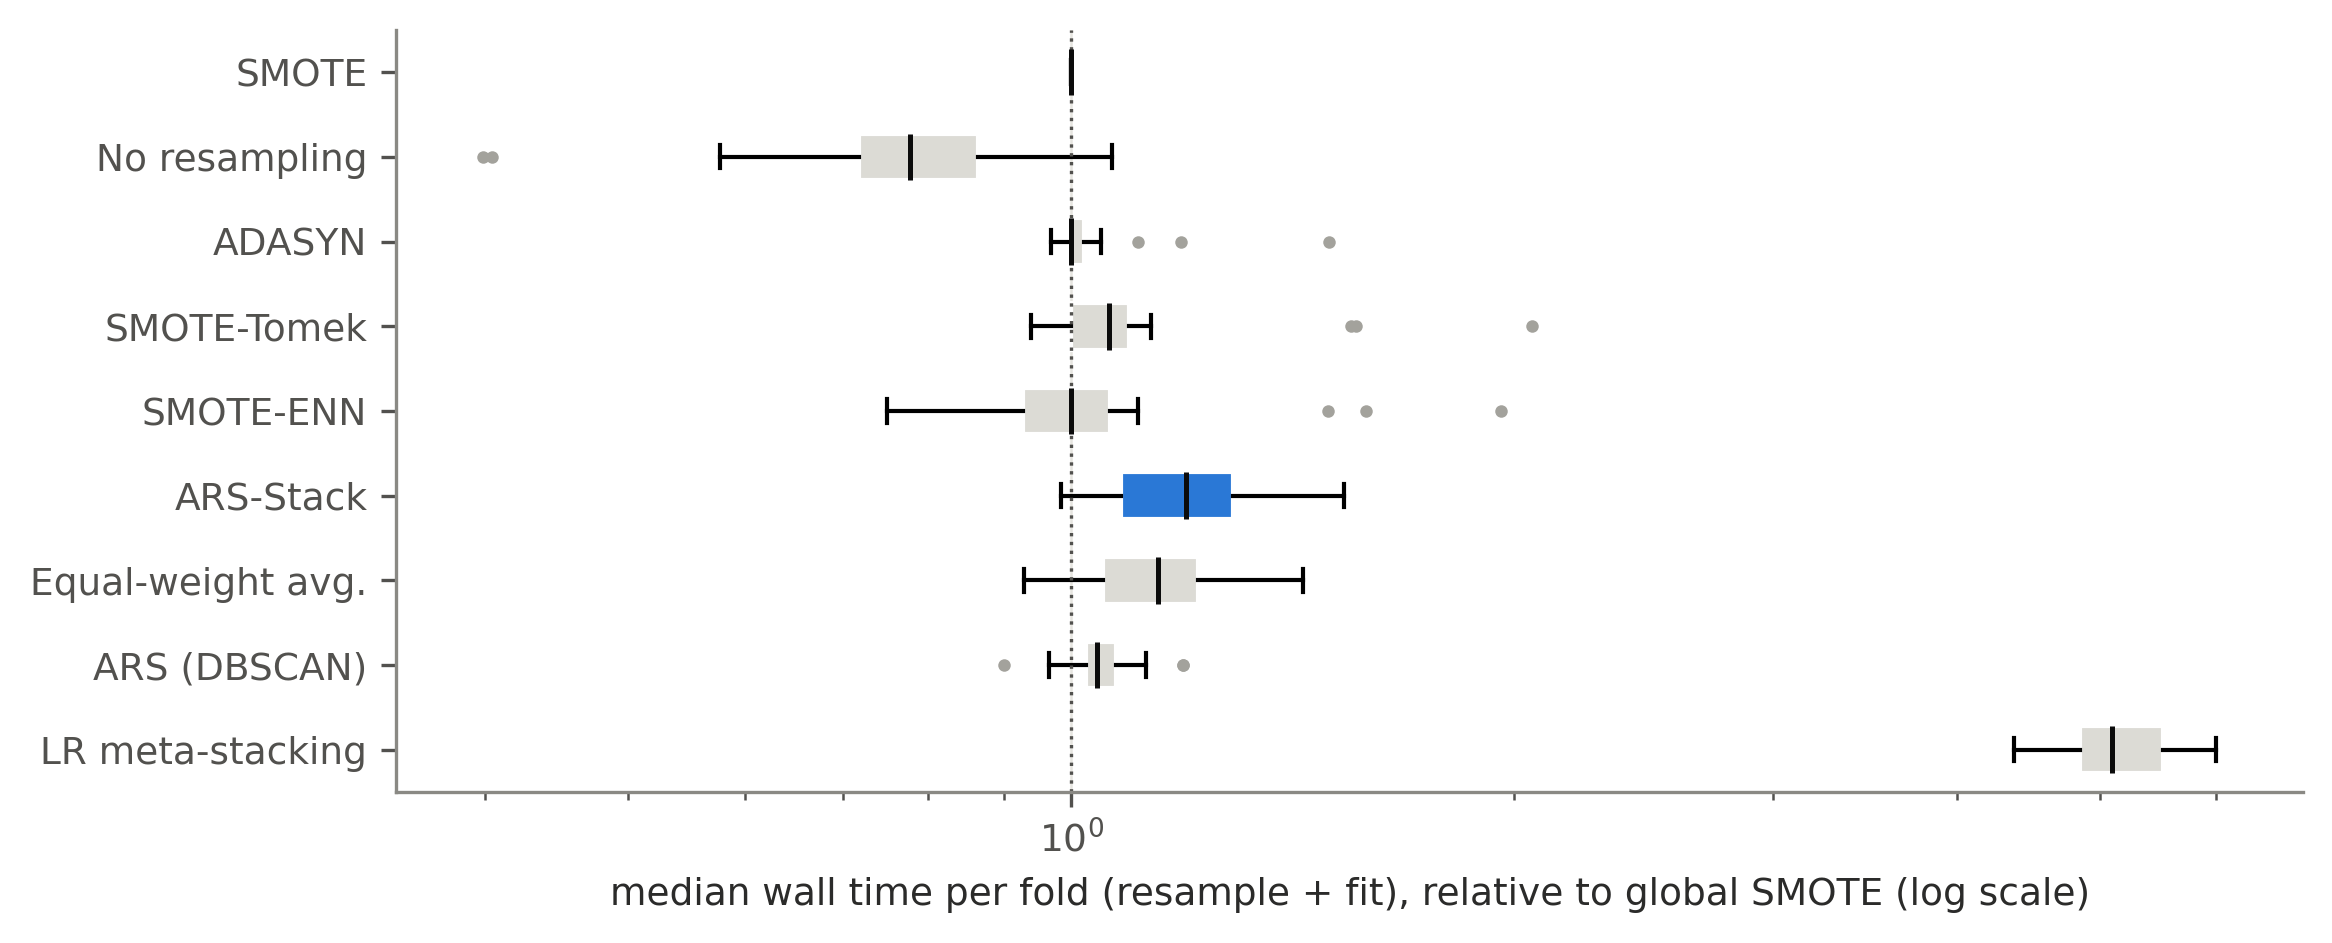
\includegraphics[width=0.85\linewidth]{fig10_cost.png}
\caption{Fold wall time (resampling + ensemble fitting) relative to global SMOTE, per dataset (log scale).}
\label{fig:cost}
\end{figure}

ARS-Stack's median fold time is $1.20\times$ that of global SMOTE (Table~\ref{tab:cost}, Figure~\ref{fig:cost}). Meta-stacking costs $5.1\times$, because it fits each learner five more times for out-of-fold predictions, and no resampling costs $0.78\times$. On the largest dataset, credit card with about 193{,}000 majority training rows, adaptive resampling takes 1.0\,s per fold. Global SMOTE-Tomek and SMOTE-ENN take 113\,s, because their nearest-neighbour cleaning runs over the full training set. Local cleaning therefore makes cleaning-based resampling about two orders of magnitude cheaper on large datasets. This is a practical benefit that holds independently of accuracy.

\subsection{Discussion}

Taken together, the results give a clear and, we believe, useful answer to the question in the title. Under a fair, budget-controlled comparison with strong gradient-boosted ensembles and a validation-tuned threshold, choosing the resampler per minority cluster \emph{does not} improve on global SMOTE, global SMOTE-Tomek, or not resampling at all. It does avoid the substantial harm of global SMOTE-ENN, and to a lesser extent of global ADASYN. Three observations explain this. (1) Local cleaning changes the training data very little. (2) The selector's choice is uniform within many datasets. (3) Tree ensembles with a tuned threshold are already robust to the residual class imbalance, which is why no resampling is competitive. This agrees with large-scale evidence that differences between good oversamplers are small \cite{kovacs2019empirical}. It also cautions against conclusions drawn from single splits and two or three datasets. Several earlier per-cluster proposals were validated that way, and our own single-split runs would have suggested different conclusions on mammography. The pre-correction pilot of this project, which oversampled the variants by different amounts, also produced apparent gains that disappeared once the comparison was controlled.

ARS-Stack is still useful in practice. It is a safe default that never fails catastrophically (it is never significantly worse than SMOTE and is significantly better than global SMOTE-ENN). It is interpretable, since every cluster's decision is logged with its scores. And it makes cleaning-based resampling cheap on large data.

% =====================================================================
\section{Limitations}\label{sec:limitations}
% =====================================================================

\begin{itemize}
  \item \textbf{Fixed selection rule.} The thresholds (0.40, 0.70, 0.75) were fixed a priori for validity and were not tuned. A selector learned from data, for example one that chooses per cluster by inner-validation performance, could behave differently. It would, however, need nested validation to avoid optimistic bias.
  \item \textbf{Few clusters.} Silhouette-based KMeans mostly returns $k=2$, which limits how much local structure the selector can exploit. We did not explore minority-specific clustering criteria or larger $k$.
  \item \textbf{Proportional allocation.} The budget is split in proportion to cluster size. Density- or difficulty-based allocation, as in K-means SMOTE \cite{douzas2018kmeanssmote}, was not combined with per-cluster selection.
  \item \textbf{Resampler pool.} Only four classical resamplers were considered. Borderline-SMOTE \cite{han2005borderline} and other modern variants were not in the pool.
  \item \textbf{Learner choice.} All variants use strong tree ensembles with threshold tuning. Resampling may matter more for weaker or linear learners, which we did not test.
  \item \textbf{Dataset scope.} 26 of 28 datasets come from public benchmark collections, and only one is multiclass. Exact duplicates were removed, so results on mammography are not directly comparable with prior work.
  \item \textbf{Statistical power.} With 15 folds per dataset and 28 datasets, small true effects (below about 0.005 AUC-PR) cannot be detected. ``No significant difference'' means practical equivalence at this resolution, not proof of exact equality.
  \item \textbf{Single hardware run.} XGBoost was trained on GPU. GPU and CPU XGBoost produce slightly different models, so exact numbers can differ marginally on CPU-only hardware.
\end{itemize}

% =====================================================================
\section{Conclusion and Future Work}\label{sec:conclusion}
% =====================================================================

We introduced ARS-Stack, which clusters each minority class, chooses among SMOTE, ADASYN, SMOTE-Tomek and SMOTE-ENN per cluster from its overlap and relative density, resamples locally under a global budget, and combines three tree ensembles with confidence weights and a tuned threshold. We evaluated it in a controlled, leakage-free study of 28 datasets, nine variants and 3{,}780 fold models with corrected statistical tests. Per-cluster selection is \emph{practically equivalent} to global SMOTE, global SMOTE-Tomek and no resampling. It is significantly better than global SMOTE-ENN, at 1.2$\times$ the cost of SMOTE. The causes are measurable: local cleaning removes almost no majority data, the selection is often uniform within a dataset, and validation-based confidence weights are nearly equal. Our results suggest that, for modern tabular learners, evaluation rigour (equal budgets, nested validation, threshold tuning and corrected multi-dataset statistics) matters more than the choice of resampler.

Future work includes: (i) a selector learned with nested validation, or a meta-learned selector based on cluster meta-features; (ii) combining per-cluster selection with difficulty-based allocation; (iii) evaluation with weaker and linear learners, where resampling is expected to matter more; (iv) more multiclass and real-world operational datasets (fraud, medical, network intrusion); (v) Bayesian correlated $t$-tests to quantify practical equivalence via regions of practical equivalence \cite{benavoli2016posthoc}; and (vi) using local cleaning as a scalable replacement for global SMOTE-ENN/Tomek on large datasets.

\section*{Data and Code Availability}
All code, configurations, per-fold results (\texttt{reports\_raw/ablation\_results/folds}), the figure- and table-generation scripts of this paper (\texttt{final\_paper/scripts}) and the environment record are included in the project repository. The pipeline is reproduced end to end by \texttt{bash scripts/run\_all.sh}.

\bibliographystyle{unsrtnat}
\bibliography{references}

% =====================================================================
\appendix
\section{Supplementary Design Diagrams}
% =====================================================================

\begin{figure}[h]\centering
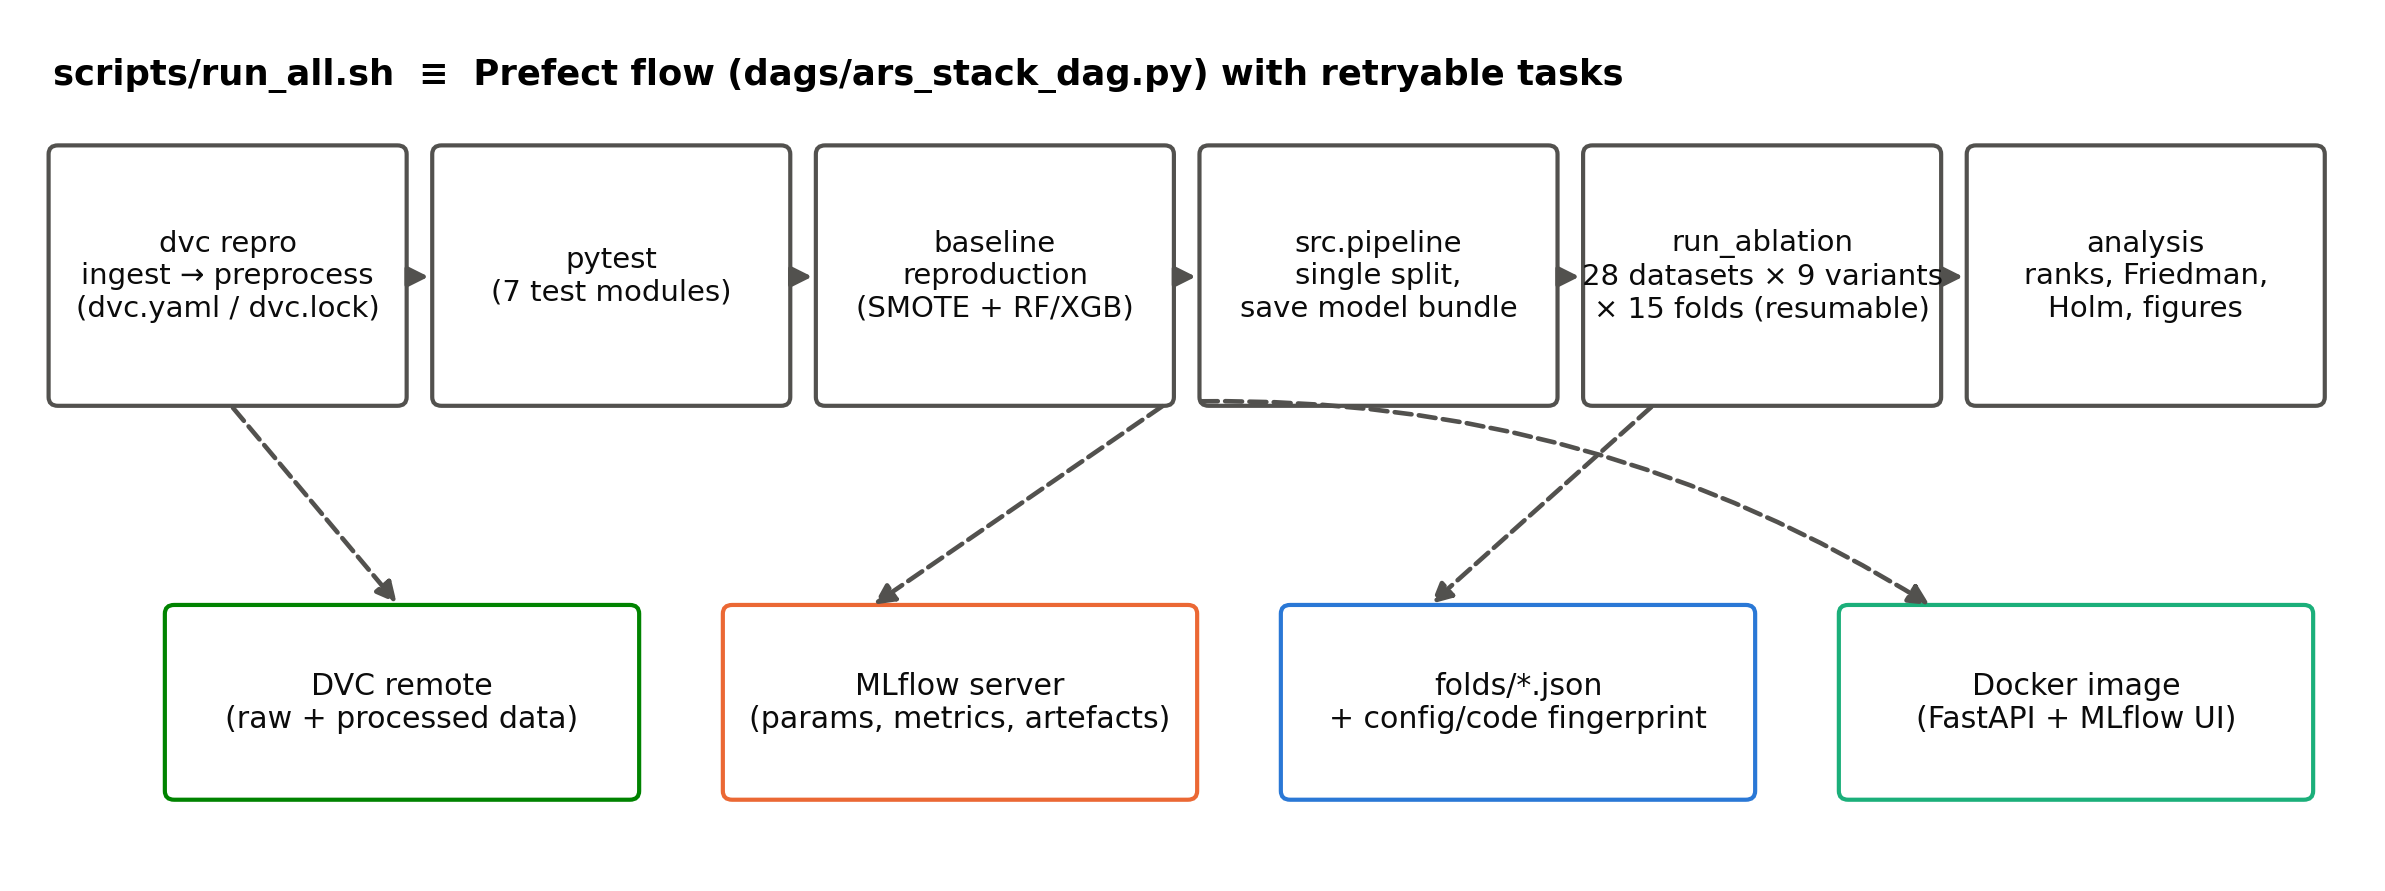
\includegraphics[width=\linewidth]{figA1_mlops.png}
\caption{MLOps and orchestration pipeline. \texttt{scripts/run\_all.sh} and the equivalent Prefect flow run the stages in order. DVC versions data, MLflow logs runs, per-fold JSON results carry code/configuration fingerprints, and Docker packages serving.}
\label{fig:mlops}
\end{figure}

\begin{figure}[h]\centering
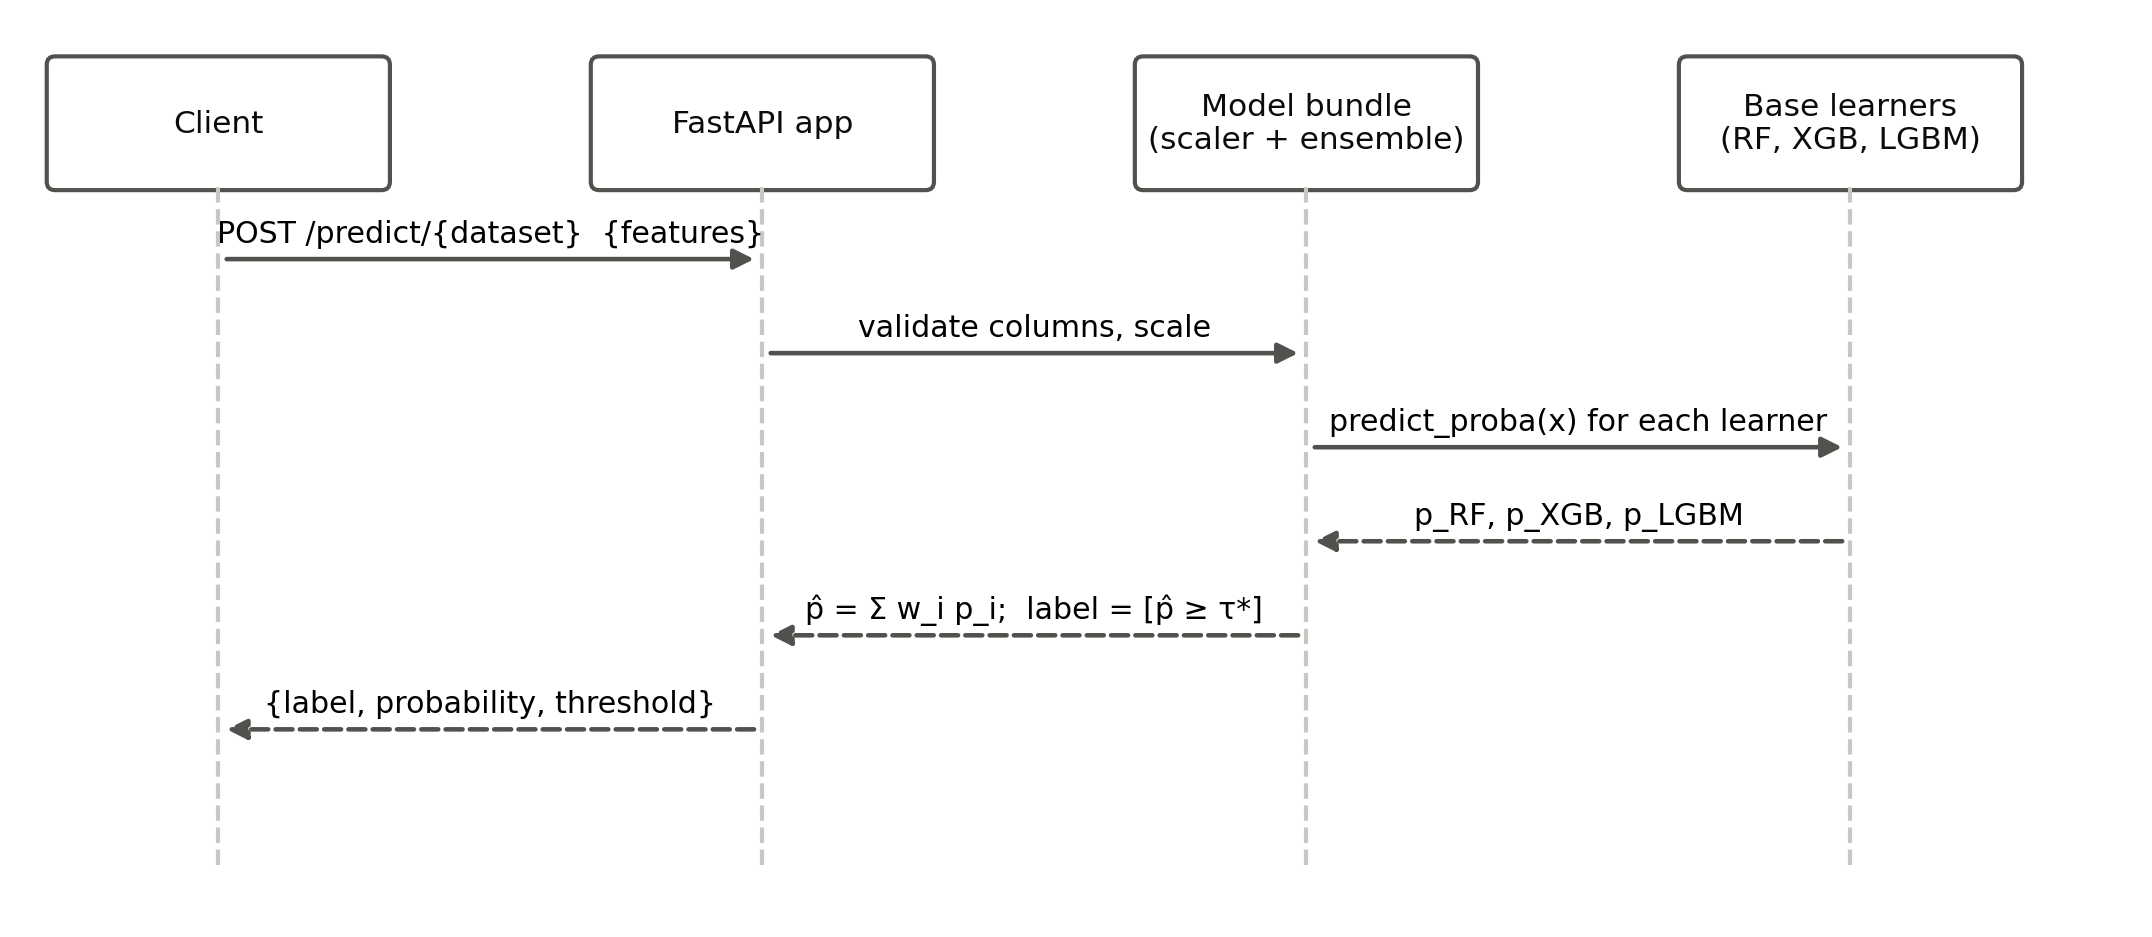
\includegraphics[width=0.92\linewidth]{figA2_serving_sequence.png}
\caption{Sequence diagram of a prediction request to the FastAPI service.}
\label{fig:serving}
\end{figure}

\begin{figure}[h]\centering
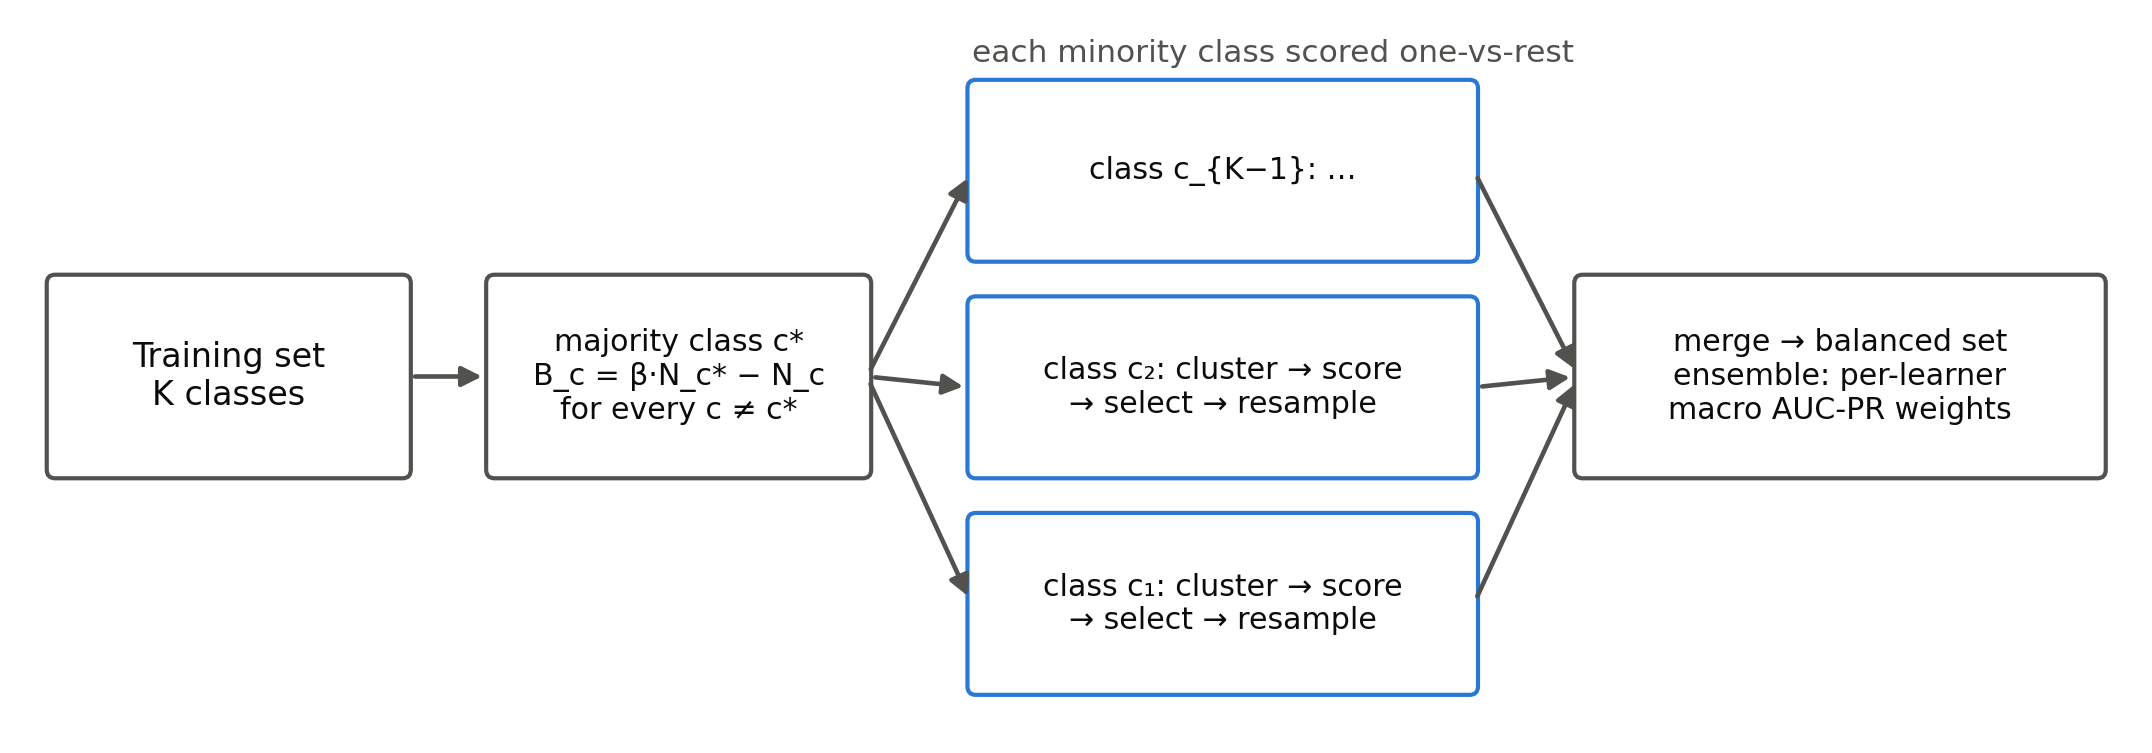
\includegraphics[width=0.92\linewidth]{figA3_multiclass.png}
\caption{Multiclass extension: every non-majority class is clustered, scored one-vs-rest and resampled with its own budget.}
\label{fig:multiclass}
\end{figure}

\clearpage
\section{Full Per-Dataset Results}

{\small\setlength{\tabcolsep}{3.5pt}
\begin{longtable}{lrrrrrrrrr}
\caption{Mean AUC-PR over 15 folds for every dataset and variant (best in bold). ARS = ARS-Stack, EqAvg = equal-weight average, Meta = LR meta-stacking, DBSC = ARS with DBSCAN, ADA = ADASYN, S-Tom = SMOTE-Tomek, S-ENN = SMOTE-ENN, None = no resampling.}\label{tab:full_auc_pr}\\
\toprule
Dataset & ARS & EqAvg & Meta & DBSC & SMOTE & ADA & S-Tom & S-ENN & None \\
\midrule
\endfirsthead
\toprule
Dataset & ARS & EqAvg & Meta & DBSC & SMOTE & ADA & S-Tom & S-ENN & None \\
\midrule
\endhead
solar\_flare\_m0 & 0.193 & 0.194 & 0.192 & 0.195 & 0.177 & 0.175 & 0.178 & \textbf{0.246} & 0.186 \\
ecoli & 0.682 & 0.684 & 0.686 & 0.682 & 0.714 & \textbf{0.719} & 0.682 & 0.651 & 0.702 \\
optical\_digits & 0.995 & 0.995 & 0.995 & 0.995 & 0.995 & 0.994 & 0.995 & 0.994 & \textbf{0.995} \\
satimage & 0.811 & 0.811 & 0.806 & 0.810 & \textbf{0.811} & 0.805 & 0.811 & 0.728 & 0.809 \\
pen\_digits & \textbf{0.999} & \textbf{0.999} & \textbf{0.999} & 0.998 & 0.998 & 0.997 & 0.998 & 0.998 & 0.998 \\
abalone & 0.290 & 0.289 & 0.291 & 0.297 & 0.302 & 0.298 & 0.305 & \textbf{0.317} & 0.297 \\
sick\_euthyroid & 0.896 & 0.897 & 0.897 & 0.898 & 0.897 & 0.896 & 0.897 & 0.868 & \textbf{0.898} \\
spectrometer & 0.865 & 0.866 & 0.865 & 0.884 & 0.878 & 0.854 & 0.885 & 0.858 & \textbf{0.913} \\
car\_eval\_34 & 0.990 & 0.990 & \textbf{0.990} & 0.990 & 0.989 & 0.990 & 0.989 & 0.973 & 0.990 \\
isolet & 0.962 & 0.962 & 0.959 & 0.962 & 0.962 & 0.960 & 0.962 & 0.867 & \textbf{0.967} \\
us\_crime & 0.550 & 0.550 & 0.549 & 0.556 & 0.546 & 0.546 & 0.548 & 0.523 & \textbf{0.594} \\
yeast\_ml8 & 0.107 & 0.107 & 0.108 & \textbf{0.112} & 0.104 & 0.103 & 0.104 & 0.105 & 0.108 \\
scene & 0.226 & 0.227 & 0.223 & 0.220 & 0.242 & 0.239 & 0.245 & 0.210 & \textbf{0.271} \\
libras\_move & 0.894 & 0.893 & \textbf{0.899} & 0.894 & 0.895 & 0.881 & 0.895 & 0.878 & 0.881 \\
coil\_2000 & 0.124 & 0.124 & 0.119 & 0.123 & 0.125 & 0.124 & 0.124 & \textbf{0.140} & 0.126 \\
thyroid\_sick & 0.946 & 0.945 & 0.944 & 0.947 & 0.946 & 0.947 & 0.947 & 0.893 & \textbf{0.954} \\
arrhythmia & 0.843 & \textbf{0.847} & 0.840 & 0.843 & 0.833 & 0.837 & 0.833 & 0.783 & 0.815 \\
wine\_quality & 0.249 & 0.249 & 0.251 & 0.265 & 0.282 & 0.274 & 0.280 & 0.271 & \textbf{0.322} \\
oil & 0.600 & 0.601 & 0.603 & 0.600 & \textbf{0.622} & 0.620 & \textbf{0.622} & 0.573 & 0.580 \\
car\_eval\_4 & \textbf{1.000} & \textbf{1.000} & \textbf{1.000} & 1.000 & 1.000 & 1.000 & 1.000 & 0.972 & 0.999 \\
letter\_img & 0.995 & 0.995 & 0.995 & 0.995 & 0.995 & 0.995 & 0.995 & 0.995 & \textbf{0.996} \\
mammography & 0.763 & 0.763 & 0.760 & 0.750 & 0.766 & 0.739 & 0.767 & 0.722 & \textbf{0.780} \\
ozone\_level & 0.356 & 0.355 & 0.355 & 0.347 & 0.369 & 0.361 & 0.369 & \textbf{0.385} & 0.321 \\
webpage & 0.814 & 0.808 & 0.788 & 0.814 & 0.814 & 0.788 & 0.814 & 0.761 & \textbf{0.855} \\
yeast\_multiclass & 0.597 & 0.597 & 0.579 & \textbf{0.601} & 0.599 & 0.586 & 0.599 & 0.566 & 0.591 \\
protein\_homo & \textbf{0.902} & 0.902 & 0.901 & 0.900 & 0.901 & 0.888 & 0.901 & 0.893 & 0.885 \\
abalone\_19 & 0.055 & 0.055 & 0.058 & 0.055 & 0.068 & 0.056 & \textbf{0.075} & 0.056 & 0.049 \\
creditcard & 0.843 & 0.842 & 0.843 & \textbf{0.844} & 0.844 & 0.836 & 0.844 & 0.830 & 0.840 \\
\bottomrule
\end{longtable}}

{\small\setlength{\tabcolsep}{3.5pt}
\begin{longtable}{lrrrrrrrrr}
\caption{Mean MCC over 15 folds for every dataset and variant (best in bold). ARS = ARS-Stack, EqAvg = equal-weight average, Meta = LR meta-stacking, DBSC = ARS with DBSCAN, ADA = ADASYN, S-Tom = SMOTE-Tomek, S-ENN = SMOTE-ENN, None = no resampling.}\label{tab:full_mcc}\\
\toprule
Dataset & ARS & EqAvg & Meta & DBSC & SMOTE & ADA & S-Tom & S-ENN & None \\
\midrule
\endfirsthead
\toprule
Dataset & ARS & EqAvg & Meta & DBSC & SMOTE & ADA & S-Tom & S-ENN & None \\
\midrule
\endhead
solar\_flare\_m0 & 0.039 & 0.039 & 0.035 & 0.029 & 0.005 & 0.006 & 0.019 & \textbf{0.075} & 0.032 \\
ecoli & 0.572 & 0.568 & 0.554 & 0.572 & \textbf{0.573} & 0.560 & 0.564 & 0.519 & 0.528 \\
optical\_digits & 0.957 & 0.957 & 0.955 & 0.959 & 0.959 & 0.948 & \textbf{0.960} & 0.954 & 0.952 \\
satimage & 0.684 & 0.685 & \textbf{0.688} & 0.684 & 0.687 & 0.679 & 0.687 & 0.615 & 0.686 \\
pen\_digits & 0.991 & 0.991 & 0.991 & 0.990 & \textbf{0.992} & 0.987 & \textbf{0.992} & 0.990 & 0.990 \\
abalone & 0.314 & 0.314 & 0.322 & 0.323 & 0.315 & 0.316 & 0.314 & \textbf{0.339} & 0.334 \\
sick\_euthyroid & 0.854 & 0.854 & 0.852 & \textbf{0.860} & 0.842 & 0.845 & 0.850 & 0.805 & 0.859 \\
spectrometer & 0.783 & 0.783 & 0.788 & 0.729 & 0.713 & 0.688 & 0.721 & 0.706 & \textbf{0.808} \\
car\_eval\_34 & 0.924 & 0.924 & 0.924 & \textbf{0.925} & 0.925 & 0.920 & 0.925 & 0.877 & 0.920 \\
isolet & 0.896 & \textbf{0.896} & 0.890 & 0.894 & 0.889 & 0.889 & 0.889 & 0.773 & 0.892 \\
us\_crime & 0.488 & \textbf{0.489} & 0.482 & 0.484 & 0.480 & 0.480 & 0.481 & 0.463 & 0.486 \\
yeast\_ml8 & 0.091 & 0.088 & \textbf{0.093} & 0.075 & 0.070 & 0.084 & 0.070 & 0.065 & 0.062 \\
scene & 0.215 & 0.216 & 0.220 & 0.211 & 0.224 & 0.224 & 0.229 & 0.197 & \textbf{0.245} \\
libras\_move & 0.622 & 0.622 & 0.622 & 0.622 & \textbf{0.676} & 0.621 & \textbf{0.676} & 0.654 & 0.599 \\
coil\_2000 & 0.122 & 0.122 & 0.112 & 0.120 & 0.126 & 0.124 & 0.129 & \textbf{0.137} & 0.136 \\
thyroid\_sick & 0.870 & 0.870 & 0.872 & 0.873 & \textbf{0.875} & 0.873 & 0.873 & 0.844 & 0.871 \\
arrhythmia & 0.686 & 0.687 & 0.695 & 0.686 & 0.690 & \textbf{0.707} & 0.690 & 0.702 & 0.667 \\
wine\_quality & 0.268 & 0.267 & 0.271 & 0.281 & 0.288 & 0.275 & 0.279 & 0.291 & \textbf{0.347} \\
oil & \textbf{0.555} & 0.546 & 0.547 & \textbf{0.555} & 0.508 & 0.550 & 0.508 & 0.543 & 0.402 \\
car\_eval\_4 & 0.939 & 0.939 & 0.939 & 0.941 & 0.932 & 0.923 & 0.932 & 0.856 & \textbf{0.942} \\
letter\_img & 0.965 & 0.965 & 0.964 & 0.964 & 0.961 & 0.965 & 0.961 & 0.960 & \textbf{0.968} \\
mammography & 0.693 & 0.688 & 0.696 & 0.676 & 0.693 & 0.694 & 0.703 & 0.654 & \textbf{0.703} \\
ozone\_level & 0.320 & 0.323 & 0.315 & 0.320 & 0.339 & 0.335 & 0.339 & 0.313 & \textbf{0.346} \\
webpage & 0.762 & 0.757 & 0.733 & 0.764 & 0.769 & 0.740 & 0.769 & 0.746 & \textbf{0.785} \\
yeast\_multiclass & 0.447 & 0.448 & \textbf{0.471} & 0.450 & 0.447 & 0.438 & 0.452 & 0.388 & 0.444 \\
protein\_homo & 0.856 & 0.856 & \textbf{0.857} & 0.855 & 0.855 & 0.847 & 0.855 & 0.841 & 0.857 \\
abalone\_19 & 0.071 & \textbf{0.080} & 0.080 & 0.071 & 0.079 & 0.045 & 0.079 & 0.071 & 0.046 \\
creditcard & 0.848 & 0.846 & 0.849 & 0.849 & 0.848 & 0.845 & 0.848 & 0.830 & \textbf{0.855} \\
\bottomrule
\end{longtable}}

\end{document}
